% This is "sig-alternate.tex" V1.9 April 2009
% This file should be compiled with V2.4 of "sig-alternate.cls" April 2009
%
% This example file demonstrates the use of the 'sig-alternate.cls'
% V2.4 LaTeX2e document class file. It is for those submitting
% articles to ACM Conference Proceedings WHO DO NOT WISH TO
% STRICTLY ADHERE TO THE SIGS (PUBS-BOARD-ENDORSED) STYLE.
% The 'sig-alternate.cls' file will produce a similar-looking,
% albeit, 'tighter' paper resulting in, invariably, fewer pages.
%
% ----------------------------------------------------------------------------------------------------------------
% This .tex file (and associated .cls V2.4) produces:
%       1) The Permission Statement
%       2) The Conference (location) Info information
%       3) The Copyright Line with ACM data
%       4) NO page numbers
%
% as against the acm_proc_article-sp.cls file which
% DOES NOT produce 1) thru' 3) above.
%
% Using 'sig-alternate.cls' you have control, however, from within
% the source .tex file, over both the CopyrightYear
% (defaulted to 200X) and the ACM Copyright Data
% (defaulted to X-XXXXX-XX-X/XX/XX).
% e.g.
% \CopyrightYear{2007} will cause 2007 to appear in the copyright line.
% \crdata{0-12345-67-8/90/12} will cause 0-12345-67-8/90/12 to appear in the copyright line.
%
% ---------------------------------------------------------------------------------------------------------------
% This .tex source is an example which *does* use
% the .bib file (from which the .bbl file % is produced).
% REMEMBER HOWEVER: After having produced the .bbl file,
% and prior to final submission, you *NEED* to 'insert'
% your .bbl file into your source .tex file so as to provide
% ONE 'self-contained' source file.
%
% ================= IF YOU HAVE QUESTIONS =======================
% Questions regarding the SIGS styles, SIGS policies and
% procedures, Conferences etc. should be sent to
% Adrienne Griscti (griscti@acm.org)
%
% Technical questions _only_ to
% Gerald Murray (murray@hq.acm.org)
% ===============================================================
%
% For tracking purposes - this is V1.9 - April 2009

\documentclass{sig-alternate}
\usepackage[normalem]{ulem}
\usepackage[usenames,dvipsnames]{pstricks}

%\usepackage{epsfig}
%\usepackage{pst-grad} % For gradients
%\usepackage{pst-plot} % For axes

\usepackage{mathtools}

\usepackage{algorithm2e}

%\usepackage[pdflatex]{graphicx}
%\usepackage{caption}
%\DeclareCaptionType{copyrightbox}
%\usepackage{subcaption}


\usepackage{multirow}

\begin{document}
%
% --- Author Metadata here ---
\conferenceinfo{CIKM}{'13}
%\CopyrightYear{2007} % Allows default copyright year (20XX) to be over-ridden - IF NEED BE.
%\crdata{0-12345-67-8/90/01}  % Allows default copyright data (0-89791-88-6/97/05) to be over-ridden - IF NEED BE.
% --- End of Author Metadata ---
\title{Efficient Temporal Synopsis of Social Media Streams}
%\title{Adapting Frequent Itemsets Mining for Social Media Text by Strengthening the Closed Property}
%\title{Strong Closure and Novelty Ranking for Efficiently Mining a Temporal Synopsis of Social Media }
%
% You need the command \numberofauthors to handle the 'placement
% and alignment' of the authors beneath the title.
%
% For aesthetic reasons, we recommend 'three authors at a time'
% i.e. three 'name/affiliation blocks' be placed beneath the title.
%
% NOTE: You are NOT restricted in how many 'rows' of
% "name/affiliations" may appear. We just ask that you restrict
% the number of 'columns' to three.
%
% Because of the available 'opening page real-estate'
% we ask you to refrain from putting more than six authors
% (two rows with three columns) beneath the article title.
% More than six makes the first-page appear very cluttered indeed.
%
% Use the \alignauthor commands to handle the names
% and affiliations for an 'aesthetic maximum' of six authors.
% Add names, affiliations, addresses for
% the seventh etc. author(s) as the argument for the
% \additionalauthors command.
% These 'additional authors' will be output/set for you
% without further effort on your part as the last section in
% the body of your article BEFORE References or any Appendices.
\maketitle
\begin{abstract}
Search and summarization of streaming social media, such as Twitter, requires the ongoing analysis of large volumes of data with dynamically changing characteristics.  Tweets are short and repetitious - lacking context and structure  - making it difficult to generate a coherent synopsis of events within a given time period.  Although some established algorithms for frequent itemset analysis might provide an efficient foundation for synopsis generation, the unmodified application of standard methods produces a complex mass of rules, dominated by common language constructs and many trivial variations on topically related results.  Moreover, these results are not necessarily specific to events within the time period of interest.  To address these problems, we build upon the Linear time Closed itemset Mining (LCM) algorithm, which is particularly suited to the large and sparse vocabulary of tweets.  LCM generates only closed itemsets, providing an immediate reduction in the number of trivial results.  To reduce the impact of function words and common language constructs, we apply a straightforward filtering step that preserves these terms only when they may form part of a relevant collocation.  To further reduce trivial results, we propose a novel strengthening of the closure condition of LCM to retain only those results that exceed a threshold of distinctiveness.  Finally, we perform temporal ranking, based on a simple information gain measure, to identify results that are particularly relevant to the time period of interest.  We evaluate our work over a collection of Tweets gathered in late 2012, exploring the efficiency and filtering characteristic of each processing step, both individually and collectively.  Based on our experience, the resulting synopses from various time periods provide understandable and meaningful pictures of events within those periods, with potential application to tasks such as temporal summarization and query expansion for search.
\end{abstract}
%\category{H.4}{Information Systems Applications}{Miscellaneous}
%A category including the fourth, optional field follows...
%\category{D.2.8}{Software Engineering}{Metrics}[complexity measures, performance measures]

%\terms{Theory}

%\keywords{ACM proceedings, \LaTeX, text tagging}
\newpage
\section{Introduction}

The nature of text in social media poses a challenge when applying traditional text mining algorithms. Text in social media is usually short, lacks context and structure, and is created at a very high rate. To tap into the benefit of social media in giving voice to ordinary people, explicit contextual information from the social graph has to be neglected. However, the collective stream from all users is overwhelmed with personal updates 
%are overwhelmingly more than 
and timely finding posts about topics of interest requires an efficient mining algorithm.
%; the bigram ``I'm'' is 
%posing a challenge on making sense of.
% The sheer volume of social media streams mandates the use of efficient algorithms, but it also and the short length of individual documents makes it possible to apply Frequent Itemsets Mining. 
The frequent itemset mining family of algorithms is very fast and efficient, however it is not readily suited for application on text. First of all, the number of itemsets mined is large and grows with the number of distinct items - which is particularly high in the text domain. 
%, specially that most of them are not interesting. 
Frequent itemset mining was originally proposed as a preliminary stage to association rules mining, which sifts through the numerous itemsets and produces a smaller number of association rules. To reduce the number of itemsets, they could be limited by setting a high frequency threshold, but this is not possible in text mining because frequencies of items follow a long tailed Zipfean distribution. %, and setting a high frequency threshold will filter out a large portion of the tail of the distribution.
Second, the high frequency of stop words and language constructs is a problem that frequent itemset mining is not equipped for handling; this doesn't happen in the domain of market basket data since the packaging of each item is not enlisted in the receipt.
%The number of itemsets produced can be reduced by setting a higher threshold on  the minimum frequency of an itemset. However, in text this threshold has to be kept low because frequencies follow a long tailed Zipfean distribution. 
%Also, the head of the distribution is made up mostly of stop words; a situation that doesn't happen in the domain of market basket data since the packaging of each item is not enlisted in the receipt!
%The first type of uninteresting itemsets is the language constructs that bear no information, such as ``such as'', and itemsets that are made up of all the different fragments of the language construct along with other items. The latter type is an artifact of itemset mining when the final itemset has such a language construct within it; for example, \{we, did, it, \#teamobama\}.
%It produces a very high number of itemsets most of them are uninteresting language constructs.
%The number of itemsets it produces is exponential in the number of items,  
%For example, one would expect that \{obama, won\}, \{sham, and, travesty, @realDonaldTrump\} and \{flag, in, her, hair\}  are  itemsets mined from Tweets posted on November 6th, 2012 using terms as items. They appear frequently in the last couple of hours of the US elections day, but they are not as frequent as \{of, the\} and other English language constructs. 
Even if a maximum frequency threshold is set, risking to filter out important itemsets, a lot of non-English language constructs will be mined because the proportion of posts in English is much higher than other languages.
Finally, there is a lot of redundancy in frequent itemsets caused by trivial differences in the language used.
 In this paper we address those problems and adapt frequent itemset mining to be effective on social media text, without degrading its efficiency.  %or relying on features of a particular language.

Unlike trending topics\footnote{http://blog.twitter.com/2010/12/to-trend-or-not-to-trend.html}  \cite{mathioudakis2010twittermonitor}, the results of frequent itemset mining include itemsets that have high frequency because of sustained, relatively high, interest as well as a spike of interest. 
% GOES TO RELATED WORK Unlike bursty events detection methods \cite{klienberg2002},
%Frequent itemsets include ``trending topics'', as well as topics that have sustained interest for longer periods of time without sudden peaks. We use the term ``trending topics'' as defined by Twitter in a blog post explaining why a topic about WikiLeaks wasn't trending as was expected by internet activists \footnote{http://blog.twitter.com/2010/12/to-trend-or-not-to-trend.html}. The blog post explains that a topic is trending if a sudden peak is detected, and links this to the change in the velocity of the conversation. Since the number of posts associated with such a trending topic must be high, Frequent Itemsets Mining will detect it. Furthermore, it detects topics that have a steady high volume of posts.
The mined itemsets provide the vocabulary associated with events and can be used in various ways for search and summarization. The collection of mining results of different epochs of time can be used for temporal query and document expansion \cite{choi2012temporal, efron2012improving}. The mining results of each epoch can be treated as a document, facilitating the creation of the ``temporal profile''\cite{jones2007temporal} of a query or a document being expanded. 
% probability of an epoch conditioned on a query can be estimated as the probability of this document conditioned on the query using any pseudo-revelance feedback method. 
% after applying appropriate weights to items.
%Liken to Rosie Jones Temporal profiles?? 
% Mention CMU and/or Glasgow's work that used pseudo-relevance feedback for Microblogs?
%
For summarization, frequent itemsets can provide a good foundation for summary creation. We refrain from using the term summary only because we don't take into account the quality measures of summaries such as coherence and cohesion. However, we propose a ranking scheme for itemsets that makes the mining results presentable to human users. The top ranked itemsets cover a variety of open topics, and within one topic different opinions are reported as separate contrastive itemsets.  
% TODO: By the date of the camera ready version, please have a url to put and tell people to go to and look! However,

\textbf{Paper outline.} The first three sections provide the necessary background for the rest of the paper. We start by discussing related work in section \ref{sec:related}, then we explain frequent itemset mining and the algorithm on which we build our work in sections \ref{sec:fim} and \ref{sec:lcm} respectively. In sections \ref{sec:socmine}, \ref{sec:strong} and \ref{sec:rank} we propose solutions to different problems faced when applying frequent itemset mining to social media text. We present the outline of those sections graphically using a frequency ordered prefix tree of the itemsets. Each path from root to a leaf in such a tree represents an Itemsets, where each itemset is ordered in non-increasing order of the frequency of items. Itemsets having the same prefix share the nodes representing this prefix. This representation is typical in the literature, and it is actually a very good representation of the frequent itemset mining problem. Figure \ref{fig:outline} shows conceptually how section  \ref{sec:socmine}, \ref{sec:strong} and \ref{sec:rank}  addresses different parts of the problem. In section \ref{sec:concfut}, we conclude and suggest future directions.

%The rest of the paper is organized as follows: We start by an overview of properties of text in social media and describe the dataset we use in section \ref{sec:socmed}. Then we explain the frequent itemset mining algorithm which we build upon in section \ref{sec:fim}. 
%In the next 3 sections we describe the adaptations we propose for making the algorithm suitable for mining social media text. In section \ref{sec:ngrams} we describe how using term N-Grams of variable lengths filters out many language constructs. In section \ref{sec:KLD} we describe the use of differential temporal features to rank interesting itemsets. In section \ref{sec:strong} we propose the strong closed property and show how to reduce the number of itemsets without loosing important ones. After that we show an example of the results of applying our methods in section \ref{sec:emperical}. In section \ref{sec:related} we discuss related work that applied Frequent Itemsets Mining on text. Finally, we finish by the conclusion and future work in section \ref{sec:concfut}.

%Mining user generated content has been a hot topic since the beginning of Web 2.0. \textbf{didn't I say I dislike such inaugrational sentences.. ehem!} Businesses are interested in getting direct insights from consumers without incurring costs for surveys, and so are governments, celebrities, and above all advertisers and market analysts. Researchers are interested because methods developed for other media does not necessarily work for social media. This is particularly correct for Twitter because of its length restriction, high volume and lack of structure. The length restriction has resulted in a very particular language use as detailed in \ref{sec:socmed}, but it seems to have also played a dual role in encouraging people to keep Tweeting about everything they do, think or feel. This resulted in a very high volume of Tweets\footnote{We receive an average of 100,000 Tweets per hour from Spritzer}, most of which is personal updates but some of which represent what is happening now. The speed of news on Twitter has been known to exceed the news on professional news agencies \cite{firststory}, and it even travels faster than earthquakes \cite{earthquake}. First stories that appear in Twitter rather than official news are covered by Twitter user present at the event, and able to provide content that cannot be acquired after the fact such as the picture of the emergency landing on the Hudson river \cite{hudson}. Such stories are noticed because of the natural collaborative filtering act of retweeting good content, and the use of the community developed convention of Hashtags. The Twitter website makes use of this by following the rise in the volume of keywords, and featuring keywords whose rise in volume accelerates more than any other. However, this does not catch topics with sustained interest. It also fails to catch important topics for which the interest is peaking within a certain niche of users. Further it is almost always polluted by uninteresting topics that are made trending. In this paper we propose...

\begin{figure*}
\centering
% Generated with LaTeXDraw 2.0.8
% Mon May 06 20:21:17 EDT 2013
% \usepackage[usenames,dvipsnames]{pstricks}
% \usepackage{epsfig}
% \usepackage{pst-grad} % For gradients
% \usepackage{pst-plot} % For axes
\scalebox{1} % Change this value to rescale the drawing.
{
\begin{pspicture}(0,-4.41)(17.948048,4.4013004)
\pstriangle[linewidth=0.04,dimen=outer](8.617168,-4.41)(17.14,8.82)
\psline[linewidth=0.04cm](0.827168,-3.59)(16.367168,-3.61)
\psline[linewidth=0.04cm,linestyle=dashed,dash=0.16cm 0.16cm](6.927168,2.57)(10.287168,2.59)
\usefont{T1}{ptm}{m}{n}
\rput(8.60748,-4.005){Items with low frequency in the data are excluded by frequent itemset mining, and hence not part of the tree}
\psline[linewidth=0.04cm,linestyle=dashed,dash=0.16cm 0.16cm](2.487168,-2.03)(14.8271675,-2.01)
\usefont{T1}{ptm}{m}{n}
\rput(3.4739747,4.075){The top of the tree is not as small as it seems.}
\usefont{T1}{ptm}{m}{n}
\rput(3.6774805,3.655){It contains a large number of itemsets which are}
\usefont{T1}{ptm}{m}{n}
\rput(2.5279298,3.295){most likely language constructs.}
\usefont{T1}{ptm}{m}{n}
\rput(12.646406,4.055){In section \ref{sec:socmine} we reduce the number of itemsets}
\usefont{T1}{ptm}{m}{n}
\rput(13.064883,3.675){made up of items from the head of the Zipfean}
\usefont{T1}{ptm}{m}{n}
\rput(2.1554394,0.675){The closed property selects }
\usefont{T1}{ptm}{m}{n}
\rput(1.9119726,0.295){non-redundant itemsets, }
\usefont{T1}{ptm}{m}{n}
\rput(3.1164062,2.295){Itemsets whose lowest frequency item is}
\usefont{T1}{ptm}{m}{n}
\rput(2.779746,1.895){within the mid-range of frequencies}
\usefont{T1}{ptm}{m}{n}
\rput(2.456875,1.515){contain interesting information,}
\usefont{T1}{ptm}{m}{n}
\rput(2.4698632,1.095){but there are too many of them.}
\usefont{T1}{ptm}{m}{n}
\rput(1.8698633,-0.105){but it is easily violated.}
\usefont{T1}{ptm}{m}{n}
\rput(13.823125,2.335){In section \ref{sec:strong} we propose the strong closed}
\usefont{T1}{ptm}{m}{n}
\rput(14.255615,1.895){itemsets, which are clusters of itemsets}
\usefont{T1}{ptm}{m}{n}
\rput(14.45792,1.495){such that every itemset makes up a}
\usefont{T1}{ptm}{m}{n}
\rput(14.534248,1.055){high proportion of the support of}
\usefont{T1}{ptm}{m}{n}
\rput(14.734629,0.695){its subsets. This eleminates cl-}
\usefont{T1}{ptm}{m}{n}
\rput(14.88792,0.295){sed itemsets generated by a }
\usefont{T1}{ptm}{m}{n}
\rput(15.1511135,-0.105){slight violation of the cl-}
\usefont{T1}{ptm}{m}{n}
\rput(15.304863,-0.525){osed condition. It also}
\usefont{T1}{ptm}{m}{n}
\rput(1.6074805,-0.505){It also doesn't solve}
\usefont{T1}{ptm}{m}{n}
\rput(1.4252441,-0.925){redundancy from }
\usefont{T1}{ptm}{m}{n}
\rput(1.0541503,-1.705){in language.}
\usefont{T1}{ptm}{m}{n}
\rput(1.3320996,-1.305){slight variations}
\usefont{T1}{ptm}{m}{n}
\rput(15.58497,-0.945){reduces redundancy}
\usefont{T1}{ptm}{m}{n}
\rput(8.506817,-2.345){After mining itemsets based on support and reducing their redundancy, we rank}
\usefont{T1}{ptm}{m}{n}
\rput(8.663008,-3.285){and features intrinsic to itemsets don't result in a good ranking. We propose a ranking scheme in section \ref{sec:rank}.}
\usefont{T1}{ptm}{m}{n}
\rput(8.621269,-2.805){the remiaining itemsets using temporal features. The majority of itemsets has low support, }
\usefont{T1}{pcr}{m}{n}
\rput(8.550049,3.535){the}
\usefont{T1}{pcr}{m}{n}
\rput(7.6920705,2.835){obama}
\usefont{T1}{pcr}{m}{n}
\rput(8.255322,1.035){won}
\usefont{T1}{pcr}{m}{n}
\rput(7.4495215,1.875){president}
\usefont{T1}{pcr}{m}{n}
\rput(10.28207,-1.625){\#mtvema}
\usefont{T1}{pcr}{m}{n}
\rput(9.840049,2.175){bieber}
\usefont{T1}{pcr}{m}{n}
\rput(10.185322,1.475){justin}
\usefont{T1}{pcr}{m}{n}
\rput(11.12207,0.655){selena}
\usefont{T1}{pcr}{m}{n}
\rput(7.958799,0.115){elections}
\usefont{T1}{pcr}{m}{n}
\rput(7.7585354,-0.925){\#elections2012}
\usefont{T1}{pcr}{m}{n}
\rput(11.554756,0.055){gomez}
\usefont{T1}{pcr}{m}{n}
\rput(6.0433006,0.615){barack}
\psline[linewidth=0.04cm,linestyle=dotted,dotsep=0.16cm,arrowsize=0.05291667cm 2.0,arrowlength=1.4,arrowinset=0.4]{->}(8.607168,4.35)(7.827168,3.05)
\psline[linewidth=0.04cm,linestyle=dotted,dotsep=0.16cm,arrowsize=0.05291667cm 2.0,arrowlength=1.4,arrowinset=0.4]{->}(7.727168,2.65)(7.367168,2.03)
\psline[linewidth=0.04cm,linestyle=dotted,dotsep=0.16cm,arrowsize=0.05291667cm 2.0,arrowlength=1.4,arrowinset=0.4]{->}(6.887168,1.63)(6.447168,0.81)
\psline[linewidth=0.04cm,linestyle=dotted,dotsep=0.16cm,arrowsize=0.05291667cm 2.0,arrowlength=1.4,arrowinset=0.4]{->}(8.427168,0.83)(8.387168,0.37)
\psline[linewidth=0.04cm,linestyle=dotted,dotsep=0.16cm,arrowsize=0.05291667cm 2.0,arrowlength=1.4,arrowinset=0.4]{->}(8.307168,-0.11)(8.3271675,-0.69)
\psline[linewidth=0.04cm,linestyle=dotted,dotsep=0.16cm,arrowsize=0.05291667cm 2.0,arrowlength=1.4,arrowinset=0.4]{->}(8.667168,2.59)(8.467168,1.25)
\psline[linewidth=0.04cm,linestyle=dotted,dotsep=0.16cm,arrowsize=0.05291667cm 2.0,arrowlength=1.4,arrowinset=0.4]{->}(8.607168,4.29)(8.547168,3.71)
\psline[linewidth=0.04cm,linestyle=dotted,dotsep=0.16cm,arrowsize=0.05291667cm 2.0,arrowlength=1.4,arrowinset=0.4]{->}(8.667168,4.35)(9.867168,2.41)
\psline[linewidth=0.04cm,linestyle=dotted,dotsep=0.16cm,arrowsize=0.05291667cm 2.0,arrowlength=1.4,arrowinset=0.4]{->}(9.227168,0.85)(10.047168,-1.39)
\psline[linewidth=0.04cm,linestyle=dotted,dotsep=0.16cm,arrowsize=0.05291667cm 2.0,arrowlength=1.4,arrowinset=0.4]{->}(11.187168,0.43)(11.347168,0.19)
\psline[linewidth=0.04cm,linestyle=dotted,dotsep=0.16cm,arrowsize=0.05291667cm 2.0,arrowlength=1.4,arrowinset=0.4]{->}(6.0871677,0.43)(5.447168,-1.03)
\psline[linewidth=0.04cm,linestyle=dotted,dotsep=0.16cm,arrowsize=0.05291667cm 2.0,arrowlength=1.4,arrowinset=0.4]{->}(10.007168,1.97)(10.267168,1.61)
\psline[linewidth=0.04cm,linestyle=dotted,dotsep=0.16cm,arrowsize=0.05291667cm 2.0,arrowlength=1.4,arrowinset=0.4]{->}(9.487168,2.01)(9.167168,1.21)
\psline[linewidth=0.04cm,linestyle=dotted,dotsep=0.16cm,arrowsize=0.05291667cm 2.0,arrowlength=1.4,arrowinset=0.4]{->}(10.467168,1.29)(10.787168,0.83)
\usefont{T1}{pcr}{m}{n}
\rput(8.892071,2.815){obama}
\usefont{T1}{pcr}{m}{n}
\rput(9.2153225,1.055){won}
\psline[linewidth=0.04cm,linestyle=dotted,dotsep=0.16cm,arrowsize=0.05291667cm 2.0,arrowlength=1.4,arrowinset=0.4]{->}(8.587168,3.29)(8.607168,2.93)
\usefont{T1}{pcr}{m}{n}
\rput(5.458535,-1.365){\#elections2012}
\usefont{T1}{ptm}{m}{n}
\rput(12.963448,3.295){distribution by flattening the distribution.}
\usefont{T1}{ptm}{m}{n}
\rput(15.73415,-1.705){in language.}
\usefont{T1}{ptm}{m}{n}
\rput(15.563946,-1.325){from variations}
\end{pspicture} 
}

\caption{Roadmap of the paper overlaid on an frequency ordered prefix tree}
%, where the higher the item in the tree the more its frequency is. The}
\label{fig:outline}
\end{figure*}

\section{Related Work}
\label{sec:related}
frequent itemset mining is a very large body of work that goes back to the early 90s. We cover the topic only briefly, as the focus of this paper is not Frequent Itemsets Mining but rather its adaptation to social media text. The original Apriori algorithm \cite{agrawal1994fast} and algorithms based on it suffer performance degradation and a big increase in memory requirement when the number of distinct items is high. This is caused by the candidate generation bottleneck as explained later. Another famous class of mining algorithms is the FP-Growth \cite{han2000mining} based algorithms. FP-Growth  skips the candidate generation step, and instead creates a succinct representation of the data as a frequency ordered prefix tree called the FP-tree. An FP-tree imposes the invariant that within a branch the frequency is non-increasing from the root down to the leaves. 
%While this class of algorithms performs better than the Apriori based ones,
The memory requirements of FP-Growth algorithm suffers from the sparsity of the data, since the data structure is succinct only if it can find common prefixes within the constraints of its invariant. 
%Also, it is not suitable for 
A less known algorithm that is robust against data sparsity is LCM \cite{uno2004lcm}, which we will describe in detail in section \ref{sec:lcm}. We use the implementation submitted to the workshop for frequent itemset mining Implementations (FIMI) '04 \cite{DBLP:conf/fimi/2004}, which is the workshop's award winner. 
%The extended LCM still beats the runner up
%and we found to perform very well on the Twitter dataset we have is LCM \cite{uno2004lcm}

%frequent itemset mining was applied to all kinds of data, including social media text. In \cite{yang2012framework}
%, which we found out about only recently, 
The problem that there are too many itemsets, with a lot of noise and redundancy, is addressed either by clustering \cite{yan2005summarizing} the itemsets or by mining only itemsets that satisfy a certain condition. The closure condition \cite{pasquier1999discovering} is a prominent condition upon which many other conditions are based. Most similar to the strongly closed itemsets we  propose are the $\delta$-covered \cite{xin2005mining} and the $\delta$-free \cite{boulicaut2003free} sets. The $\delta$-covered condition is exactly the opposite of the strong closure condition, and it ``relaxes the closure condition to further reduce pattern set size'' \cite{liu2012finding}. The $\delta$-free condition is like the strongly closed condition but it is used to eliminate different itemsets, since the motivation is to provide a compressed representation of itemsets by sacrificing support information. 
%In fact, t

The motivation of most of the work in finding representative itemsets is compressing itemsets mined from a general dataset. This leads to decisions different than what  are made in order to find the most informative itemsets mined from text.
For example, in \cite{li2010mining} itemsets are mined from paragraphs of newswire text, and used to determine term weights for query expansion. Improvements in performance have been achieved by using itemsets known to come from a training set of related documents as well as ones from unrelated documents. In \cite{laumicroblog}, similar methods of term weighting were used in pseudo-relevance feedback  for Twitter search, and achieved improvements on a weak baseline. \textbf{should I include the afore mentioned attempt?}
On the other hand, in %a recent work 
\cite{yang2012framework} LCM is also used to mine Twitter posts and then a few itemsets are selected as a ``summary'' of the data, but they are selected according to their utility in a
%, similar to our work, the authors make an effort to select only a few frequent itemsets. However, they address the problem as a stream compression problem and they select itemsets based on utility in their proposed
lossy compression algorithm.
%, SPUR. SPUR is based on representing transactions as itemsets that cover them, and it might introduce false positives and negatives. The algorithm could meet the desired  constraints on memory consumption (set at 20MB) and on processing data as a stream, but there was no justification why such tight constraints should be set. On the other hand, 
The quality of the summary seems to be affected by the choice of utility function, but the only assessment made about this was showing that the actual transactions can be reconstructed from the summary with an accuracy that is expected to be high if the Tweet contains ``both recent and frequent keywords''. In the experiments, non-negative matrix factorization is used to extract topics from parts of the summary matching a query (world cup) and specific time intervals (before certain matches). It is unclear whether the raw summary would cover a variety of topics, specially non-trending ones, and no ranking scheme was shown to pick interesting topics without specifying a query. Moreover, the data is preprocessed by stemming and stop words removal, which should require a language identification component upstream but it is not discussed.
%the algorithm is used to summarize Tweets matching the query ``world cup'' from specific time intervals (during the world cup), then nonMatrix Factoization but the top chosen patterns are not compelling. 

%There are two other works from the same author, but their results are not good.. should I cite? Pattern Cooccurrence Matrix and Queensland in TREC Microblog 2011



\section{frequent itemset mining}
\label{sec:fim}
\subsection{Preliminaries}
Traditionally, frequent itemset mining is applied to a \emph{database} of \emph{transactions} made at a retail store. This terminology is suitable for market basket data and we will stick to it out of convention, even though we are mining text where the terms corpus and document are normally used. Because of the dynamic nature of social media, rather than giving the whole database as input to mining algorithms, the input is an \emph{epoch} of data; data with timestamps within a certain period of time. The epoch's \emph{span} is the length of this period in hours, and the \emph{volume} at this epoch is the number of transactions in the epoch divided by its \emph{span}.

A \emph{frequent itemset} is a set of items that occur together a number of times higher than a given threshold, called the \emph{support} threshold. We also adapt the support threshold to the dynamicity of the \emph{volume} at different times of the day. We define the \emph{minimum support threshold} as the threshold at the hour of the least \emph{volume} during the day.  The \emph{minimum support} is supplied as an absolute number, $a$, and then converted to a ratio, $\alpha = \frac{a}{avg(volume_{daily-minimum})}$.
%\begin{equation}\alpha = \frac{a}{volume_{daily-minimum}}\end{equation}
%The actual support threshold used for mining any given \emph{span} of time is thus $\alpha$ multiplied by the number of transactions in the \emph{epoch}. 
The actual support threshold used for mining any given epoch is thus $\alpha$ multiplied by the \emph{epoch}'s \emph{volume}. 

%frequently; for example, when mining Tweets posted on November 6th, 2012 using terms as items, the set \{of, president, states, the, united\} is a frequent itemset (ordered lexicographically). Traditionally, frequent itemset mining is applied to a \emph{database} of \emph{transactions} made at a retail store. This terminology is suitable for market basket data, but as we are mining social media text we use the term \emph{document} instead of transaction. It is noteworthy that this term is used as a matter of convention, yet our methods are tailored for the short ``documents'' typical of social media as described earlier. Because of the dynamic nature of social media, we call the input to a mining algorithm an \emph{epoch} of data rather than a database. An epoch of data is all documents posted in a certain period of time, the length of this period is the epoch's \emph{span}.
% in a dynamic "corpus" typical of social media as described earlier.\emph{corpus} instead of database

%The \emph{support} of an itemset is the number of times it appears, as a ratio of the number of documents in the epoch. The \emph{minimum support} is a threshold separating \emph{frequent} itemsets from \emph{infrequent} ones. Even though selecting itemsets based on their frequency of appearance was criticized in the domain of market basket data because it generates obvious itemsets, it makes sense in the domain of social media because this acts precisely as a collaborative filter. 

We now introduce the notation used in this paper:

\begin{itemize}
\item $W = \{w_1,w_2,.., w_n\}$: The set of all items (vocabulary).
\item $t_a = \{w_{a1},w_{a2},..\}$: A transaction made up of as a set of items, not necessarily terms. Each transaction has a sequential id denoted by the subscript letter.
\item $E^{span} = \langle t_a, t_b, ..\rangle$: An epoch of data of a certain span, such as an hour, made up of a sequence of transactions.
\item $s \subset I$: An itemset, its support is given by $|T_s|$.
\item $T_s = \{t: s \subseteq t\}$: All transactions containing itemset s.
\item $|.|$: Cardinality operator; gives the size of the operand.
%\item $|.| = \sum_{x \in .}{|x|}$: The Manhattan norm.

\end{itemize}

\subsection{Background}

The two basic operations of frequent itemset mining algorithms are \emph{Candidate Generation} and \emph{Solution Pruning}. The original Apriori algorithm by Agrawal et al. \cite{agrawal1994fast} generates candidates of length \emph{K} (\emph{K}-itemsets) by merging frequent itemsets of length \emph{(K-1)} (\emph{(K-1)}-itemsets) that differ in only 1 item, usually the last item given a certain total ordering of items. By using only frequent  \emph{(K-1)}-itemsets for generating candidate \emph{K}-itemsets a lot of possible \emph{K}-itemsets are implicitly pruned, based on that all subsets of a frequent itemset has to be frequent (the Apriori property). This still generates a very large number of candidates, specially in early iterations of the algorithm. Consider, for example, the generation of candidate \emph{2}-itemsets from a database. This requires producing all unordered pairs of \emph{1}-itemsets (terms), after pruning out rare ones with frequency less than the support threshold. In many domains, including text mining, the number of fequent \emph{1}-itemsets is large enough to prohibit generating a number of candidates in the order of this number squared. In text mining, a rather low support threshold has to be used, because the frequency of terms follow a long tailed Zipfean distribution.

\section{Basic Algorithm}
\label{sec:lcm}
To overcome the bottleneck of \emph{Candidate Generation}, many algorithms are proposed to take hints from the transaction space rather than operating blindly in the item space. Some algorithms do that by traversing a data structure representing the transactions \cite{han2000mining}, and others do that by generating itemsets having % each based on 
a certain property that helps pruning out more candidates. In this paper we expand on LCM \cite{uno2004lcm}, an algorithm based on a property of a class of itemsets called \emph{Closed Itemsets} \cite{pasquier1999discovering}. A closed itemset contains any item that is present in all the transactions containing this itemset. A formal definition of closed itemsets is given in equation \ref{eq:Closed}: 

\begin{equation}\label{eq:Closed}\mathcal{C} = \{s_c:\, \nexists \, s_d \, where \, s_c  \subset s_d \, and \, |T_{s_c}| = |T_{s_d}|\}\end{equation}

The properties of Closed Itemsets are the following:
\begin{enumerate}
\item Adding any item to a closed itemset reduces its support. 
\item A subset of a closed itemset is not necessarily closed, but one or more closed subset must exist for any itemset (formally this could be the empty set, given that any item that appears in all transactions is removed in a preprocessing step). 
\item If a closed \emph{K}-itemset can be extended any further then one of its supersets will be closed, however not necessarily a \emph{(K+1)} superset. Itemsets that cannot be extended any further are called \emph{Maximal Itemsets}, and they are a subclass of closed itemsets.
\end{enumerate}

Besides being much smaller than the solution space of frequent itemsets, the solution space of closed itemsets can be navigated efficiently. By using an arbitrary total ordering of items, any closed itemset can be considered an extension of exactly one of its subsets. Thus, only this subset is extended during candidate generation. All the other subsets do not need to be extended by items that would lead to the longer closed itemset.  This is called \emph{Prefix Preserving Closure Extension (PPC-Extension)} and it is proposed and formally proved in \cite{uno2004lcm}. This is achieved by following three rules, which we state after a few definitions to facilitate their statement. First, an item is \emph{larger/smaller} than another item if it comes later/earlier in the total ordering. This terminology comes from that LCM is most efficient if the items are ordered in ascending order of their frequency. Second, the \emph{suffix} of an itemset is one or more items whose removal does not result in an itemset with higher support. Notice that they will necessarily be at the end of the itemset, regardless of the total ordering. Finally, we call the first item added to the suffix of the itemset its \emph{suffix head}. With this terminology, the rules for \emph{PPC-Extentsion} are:
\begin{enumerate}
%\item The total ordering is used to generate \emph{1}-itemsets 
\item An itemset can be extend only by items \emph{larger} than its \emph{suffix head}. Extending by \emph{smaller} items will lead to closed itemsets already generated.
\item After forming an itemset $S$, add to its \emph{suffix} all items whose frequency within $D_S$ is equal to $|D_S|$. %Maintain the order of addition within the suffix.
%\item If the order of the suffix does not follow the total ordering, prune this solution branch. 
\item If any item in the \emph{suffix} is \emph{smaller} than the suffix head, prune this solution branch. All closed itemsets within this branch have already been generated.
%\item When extending by an item that has \emph{friends}, within the context of the current itemset, all \emph{friends} are added since they appear only together.  
%\item Skip any extension item that has a \emph{friend} item \emph{larger} than it. This rule can be reversed.
%, possibly affecting performance.
%, depending on what would result in smaller merges. 
%The solutions generated by adding this \emph{smaller} item to the itemset will be generated when adding the \emph{larger} item to the itemset. %, and thus it will be redundant to 
\end{enumerate}
 

%Second, an item is a \emph{friend} of another item in a certain context if they both appear only together in this context. A context is a subset of the database, for example the transactions that contain a certain item. Finally, the smallest item in the friends of the last item of the itemset is called the \emph{suffix head} of the itemset.

%Finally, the  maximum item whose removal does not change the support of an itemset is called the \emph{core item} of the itemset. It is usually the pre-last item, but not necessarily so if the last item has friends. 
% (which is equivalent to the item's postings list in an inverted index). 

Table \ref{table:PPCExample} is an example of how \emph{PPC-Extentsion} is used to generate closed itemsets starting from the  \emph{1}-itemset `barack'. The upper table enumerates $D_{barack}$. %, the documents containing `barack'. 
The lower table shows steps of itemsets generation. The current solution along with its frequency is in column 2, solutions marked by an * are the closed itemsets emitted. All possible extension items and their frequencies are in column 3 with the one being considered bolded. Column 4 is a comment explaining the step. At each step, a pass is done on $D_{itemset}$ to enumerate and count possible extension items.
% After the counting step, the rules of PPC-Extension are followed to decide whether to output an itemset as a closed one or not. 
To enforce a support threshold infrequent extension items are removed, but in this example there isn't such a threshold. Notice that the number of steps is linear in the number of closed itemsets, and the only additional storage required besides the storage of the documents is that of the possible extension items. Of course this is a simplified example, but it shows in essence how LCM achieves its low run time and memory requirements. We refer the interested reader to \cite{uno2004lcm} for a theoretical proof that the algorithm runs in linear time in the number of closed itemsets, and that this number is quadratic in the number of transactions. Performance on a real data set is shown in section \ref{sec:socmine}. We proceed by describing how to implement this algorithm using an inverted index.

%all closed itemsets were generated in 5 steps (not counting steps shown only for explanation), with only one redundant step  
%The most important contribution of LCM is that it generates closed itemsets from 

\begin{table*}
\centering
\begin{tabular}{|c|p{5cm}||c|p{5cm}|} \hline
Doc. Id & Document & Doc. Id & Document\\\hline
a& barack \& mitt & b & brack obama \& mitt romney  \\\hline
c& brack obama \& romney & d & brack obama  \\\hline
\end{tabular}
\begin{tabular}{c}
Documents (two per row)\\\\
\end{tabular}
\begin{tabular}{|c|p{4.5cm}|p{5cm}|p{6cm}|} \hline
Step&Current Solution&Possible Extension Items&Comments\\ \hline
1& \{barack\} (4)* & \textbf{mitt} (2), obama (3), romney (2) & Items are ordered lexicographically\\ \hline
2& \{barack,mitt\} (2)* & \textbf{obama} (1), romney (1) & Extension items reenumerated \& counted\\ \hline
%`obama' and `romney' are \emph{friend} items in this context. \\ \hline
%3 & \{barack, mitt\} (2) & \sout{obama} $\rightarrow$ \textbf{romney} & Rule 3: `obama' skipped. If ordered by \\\hline
3 & \{barack,mitt,obama\} (1) & romney (1)                       & Rule 2: `romney' appears in all $D_{itemset}$\\\hline
%freq. of `romney' = $|D_{itemset}|$ \\\hline
4 & \{barack,mitt,obama,romney\}(1)* & & Rule 2: `obama'  is the \emph{suffex head} \\\hline
5 & \{barack\} (4) & mitt (2), \textbf{obama} (3), romney (2) & Nothing more to add, back to `barack' \\\hline
%, extension item `obama'. \\\hline
6 & \{barack, obama\} (3)* & \sout{mitt} (1), \textbf{romney} (2) & Rule 1: skipping `mitt', adding `romney' \\\hline
7 & \{barack, obama, romney\} (2)* & \sout{mitt} (1) & Rule 1: Nothing more to add. \\\hline
8 & \{barack\} (4) & mitt (2), obama (3), \textbf{romney} (2) & Back to `barack', adding `romney' \\\hline
9 & \{barack, romney\} (2) &  \sout{mitt} (1), obama (2) & Rule 2: add obama to suffix after `romney' \\\hline
10 & \{barack, romney, obama\} (2) &  \sout{mitt} (1)  & Rule 3: suffix isn't ordered, prune solution\\\hline

\end{tabular}
\begin{tabular}{c}
Closed itemsets containing `barack'
\end{tabular}
\caption{Generation of closed itemsets by Prefix Preserving Closure Extension}
\label{table:PPCExample}
\end{table*}

\subsection{Implementation details}
We show in algorithm \ref{algo:lcmix} how to implement LCM and PPO-Extension using an inverted index. The algorithm takes as input an epoch of data and a support threshold as a ratio $\alpha$. It outputs the closed itemsets with support more than the threshold. Along with each itemset in the solution, it also outputs the transactions in which it occurs - which is represented as $\langle items, |T_{itemset}| \rangle$. The symbol $\succ$ denotes that the lefthand side  succeeds the righthand side in the total ordering.

The algorithm also lends itself to distributed implementations easily. For example, a Map/Reduce implementation is easy since the only operations are counting (line 14) and projection (line 22). However, the fast execution time and the low memory requirements of the algorithm makes it possible that a distributed implementation will cause an overhead. In the implementation shown, it is not necessary that the index's tokens list follow the total ordering; all itemsets of length 1 will be considered anyway. 
%The first line assumes that any item present in all documents is removed in a preprocessing step
%By tracing the call tree of the recursive implementation shown, we 

\begin{algorithm}
\SetAlgoLined
\LinesNumbered
\SetKwProg{Fn}{Function}{ is}{end}
\KwIn{$\alpha$: Dynamic support ratio}

\KwData{E: Epoch of data}
\KwResult{C: Closed itemsets having support $\alpha$ within E}
C $\gets \{\langle \emptyset, E\rangle\}$ \tcp*{$\emptyset$ is a closed itemset!}
X $\gets$ Inverted index of E\;
%(\tcp{follow total ordering})
\ForEach{$w \in X.tokens$}{
	$T_{\{w\}} \gets$ X.postingsList[$w$]\;
	\lIf{$|T_{\{w\}}| \geq \alpha \frac{|E|}{E.span}$}{
		LCM($\{w\}, w, T_{\{w\}}$)
	}
}
\Return{C}\;

\Fn{LCM(s: Current itemset,   $w_{sh}$: Suffix head, \\ $T_s$: Transactions (Tweets) containing s)}{
	frequency[$1 \ldots w_n$] $\gets$ 0\;
	suffix $\gets \{ w_{sh}\}$\;
	\ForEach{$t \in T_s$}{
%(\tcp*{Documents can be stored according to total ordering})
		\ForEach{$w \in d$}{ % such that $i \succ i_{sh}$}{
			frequency[$w$]++\;
			\lIf{frequency[$w$] $ = |T_s|$}{
				suffix.add($w$)	
			}
		}
	}
	\lIf{$\exists v \in suffix: w_{sh} \succ v$ }{
		\Return
	}
	C.add($\langle s \cup suffix, T_s\rangle$)\;
	\ForEach{$v \succ w_{sh}$ and $v \notin $ suffix}{
		\If{frequency[$v$] $\geq \alpha \frac{|E|}{E.span}$}{
			$D \gets T_s \cap v$	\tcp*{Results of query $s$ AND $v$}
			LCM($s \cup suffix \cup \{v\}, v, D$) 
		}
	}
}

\caption{LCM Frequent Itemsets Mining}
\label{algo:lcmix}
\end{algorithm}

%The algorithm described works well on the sparse data typical to text mining. 
%FIMI??
%In the next few sections we will see how to make the efficient fre also effective.

\section{Mining social media}
\label{sec:socmine}

Throughout this paper we use data we have been collecting from the Twitter public stream\footnote{https://dev.twitter.com/docs/streaming-apis/streams/public} as of October 1st, 2012. 
% at 00:00 HST. We use Hawaii Standard Time as our reference 
We use only Tweets written in Latin script to facilitate tokenization using white space and other word boundaries. We collected only the Tweet text to avoid reliance on any features specific to a certain social medium, and make the algorithms applicable to other media where text is short such as comments and Facebook or Google+ status updates. The only preprocessing performed was removing duplicate original Tweets (not retweets) using a Bloom filter. This removes spam Tweets sent by BotNets, such as advertisements about Raspberry Ketone diets.

We apply the algorithms to epochs of data, so they are not strictly stream processing algorithms. However, we regard the process as mining a sliding window that is moved forward by time steps of short span. The time step must be longer than the time needed to mine an epoch of data, and the performance of our algorithms makes it possible to use a time step of a few seconds for epochs up to a day long. Figure \ref{fig:runtimeEpochs} shows the runtime of LCM on epochs of increasing length, and we will show in section \ref{sec:bounding} that our extensions don't degrade the performance. The times reported in figure \ref{fig:runtimeEpochs} are averages across all epochs of the specified length in the months of October, November and December, using a time step that is half the epoch length. The variance is very low and the confidence bands are not shown because they appear as dots on top of the bars. 
 %much shorter than time needed for human perception. 
% arbitrary span is processed in much less time than its span.

The support threshold used throughout this paper, unless otherwise specified, is $\alpha=0.0002$. This is determined as follows: We picked a topical term that is known to  steadily  appear with a rather high frequency, and is talked about in all languages; `obama'. The maximum likely hood estimate of the probability of the term `obama' within the whole collection of Tweets is 0.0001. Since the average number of Tweets per hour is 100000, so the term `obama' is expected to appear 10 times per hour on average. Thus, we use a minimum support threshold of 10, which translates into $\alpha = 0.0002$.

In the rest of this paper we mine epochs of 1 hour span. The reason behind this choice is an observation that the number of closed itemsets mined from epochs of span 1 hour or more, at the same support threshold, remains that same. This indicates that itemsets mined from shorter epochs of social media text are not included in the results of mining longer epochs. 
%We will show that itemsets mined from epoch of span 1 hour are not only languag
Therefore, the epoch span should be minimized. However, when the epoch span is shorter than an hour the frequency required to surpass the support threshold becomes very low, and number of mined itemsets increases because a lot of noise itemsets are mined.

\begin{figure}
\centering
% Generated with LaTeXDraw 2.0.8
% Wed May 01 10:13:00 EDT 2013
% \usepackage[usenames,dvipsnames]{pstricks}
% \usepackage{epsfig}
% \usepackage{pst-grad} % For gradients
% \usepackage{pst-plot} % For axes
\scalebox{.4} % Change this value to rescale the drawing.
{
\begin{pspicture}(0,-5.61)(19.94,5.61)
\rput(9.97,0.0){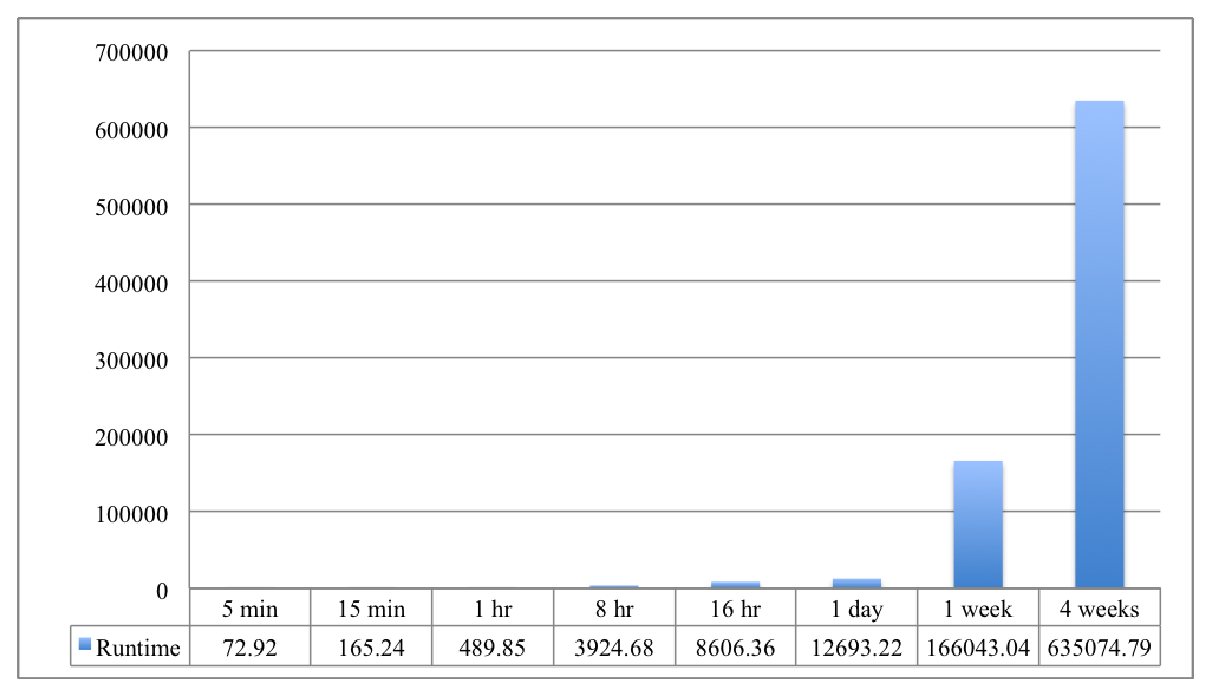
\includegraphics{runtime_different-epoch-spans_bar-table.eps}}
\rput(9.8,1.44){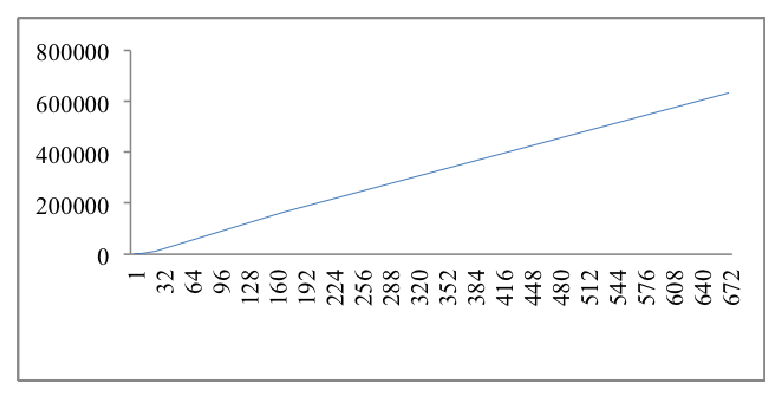
\includegraphics{runtime_different-epoch-spans_line.eps}}
\usefont{T1}{ptm}{m}{n}
\rput{90.15449}(0.96138316,-0.45039606){\rput(0.6871191,0.225){\LARGE Time in milliseconds}}
\usefont{T1}{ptm}{m}{n}
\rput(10.130039,-0.925){\Large Epoch span in hours}
\end{pspicture} 
}
\caption{Mean runtime at different epoch spans}
\label{fig:runtimeEpochs}
\end{figure}

\subsection{Mining term N-Grams}
\label{sec:ngrams}

A large number of itemsets are language constructs that bear no information, such as ``such as''.  By treating sequential language constructs, and any other multiword expression, as one item we eliminate a large number of such itemsets. Actually, we also eliminate itemsets that are made up of all the different fragments of the language construct along with other items; for example, \{we, did, it, \#teamobama\} can produce 10 other combination of length 2 or more. There are many measures of association that can be used to detect multiword expressions, but each measure is good only under certain conditions and has special properties \cite{ramisch2012broad}. We experimented with various measures, and in fact we found out that a very good measure for identifying multiword Named Entities is Yule's Q; a measure of association and disassociation derived from the odds ratio. However, we have finally found that for the purpose of preprocessing before Frequent Itemsets Mining what works best is tokenizing the documents into term N-Grams with varying N. 

We start by tokenizing into unigrams, and counting their frequencies. Then we use the probability of the same word used to determine the support threshold, $P(`obama') = 0.0001$, and assume that this is where the head of the Zipfean distribution starts. For each unigram belonging to the head, we create two term bigrams by attaching to it the unigrams before and after it. We repeat this foreach N $\ge$ 1 by creating two (N+1)-Grams for all N-Grams with probabilities above the threshold until there are no more such N-Grams. We do not prevent overlap, because there is no guarantee that the N-Gram created makes any sense. At each N, the probability threshold is adjusted to account for the increase in the number of tokens and the overall increase in the grand sum of counts, since each high frequency N-Gram is replaced by two lower frequency ones. Let the original probability threshold be $\eta$, then the adjusted $\eta_N$ is:
\begin{equation}\eta_N = \eta * \frac{\sum_{\{w:\, w \,\in\, W\, and\, w.length \,\le\, N\}}{freq(w)}}{\sum_{\{v:\, v\, \in\, W \,and \,v.length\,=\,1\}}{freq(v)}}\end{equation}
% At each N, the probability threshold is adjusted by the ratio of the sum of the counts of all terms of length up to (N+1), to the the sum of the counts of all terms of length up to N-Gram.

%as described above 
%Throughout the discussion above, 
%In the next few sections we will look at ways to reduce the number of itemsets produced and filter out uninteresting ones. 
%counts the support of itemsets 
%While extremely fast, Frequent Itemsets Mining produces numerous itemsets that are not interesting. Actually it was originally proposed as a preliminary stage to Association Rules Mining, which sifts through the relatively high number of itemsets and produces a smaller number of association rules. The first type of uninteresting itemsets is the language constructs that bear no information, such as ``such as'', and itemsets that are made up of all the different fragments of the language construct along with other items. The latter type is an artifact of itemset mining when the final itemset has such a language construct within it; for example, \{we, did, it, \#teamobama\}.
% One possibility to get rid of such itemsets is to mine itemsets 
% and might produce wrong results otherwise
%If we can treat sequential language constructs, and really any other multiword expression, as one item we reduce the number of itemsets produced in these two ways. %just described.
%itemsets that are parts of it will not be produced, and fragments of it along with other itemsets in the rest of 
%they will not be produced as itemsets (since we produce only itemset of length 2 or more). 



%We start by tokenizing into unigrams, then we
%producing term N-Grams from the window surrounding any token 
%create two term bigrams for each unigram appearing with a probability above a certain threshold, $\eta$, by attaching to it the unigrams before and after it. We do this recursively by increasing N and creating two (N+1)-Grams for each N-Gram above the threshold until there are no more N-Grams above the threshold. 
%At each value of N, the threshold $\eta$ is adjusted by the ratio of the number of tokens of length up to N and the number of unigrams; $\eta_{N} = |\eta_1| * \frac{| I_{N}|}{|I_{1}|}$.
% thus flattening the Zipfian distribution a little. 
%Following we present an example of tokenizing ``Barack Obama president of the United States'':

%\begin{enumerate}
%\item First the tokens will be: \texttt{`barack', `obama', `president', `of', `the', `united', `states'}. 
%\item Assume that after tokenizing the whole epoch we find that the probability of \texttt{`obama', `of'} and \texttt{`the'} within the current epoch is more than $\eta$. Therefore the tokens are changed to: \texttt{`barack',  `barack + obama', `obama + president', `president', `president + \\of', `of + the', `the + united', `united', `states'}.
%\item Assume that the bigrams  \texttt{`barack + obama'} and \texttt{`of + the'} still appear with a probability higher than %the adjusted
%$\eta$. Therefore trigrams are generated by attaching the unigrams before and after them, and the tokens become: \texttt{`barack',  `barack + obama + president', `obama + president', `president', `president + of', `president + of + the', `of + the + united', `the + \\united', `united', `states'}
%\item At N=3, we find that no trigrams still appear with probability greater than $\eta$, and thus terminate.
%\end{enumerate}

%Note that in the above procedure we didn't prevent overlap, because there is no guarantee that the N-Gram created makes any sense. The goal is to create a single unit out of frequent sequences and this is achieved because an N-Gram keeps growing as long as it is frequent.
%, which will stop as soon as a unigram that is not part of the expression is attached to it. We can look at this as flattening the Zipfian distribution by creating more tokens with less frequency each, but the distribution of the input doesn't affect the results of itemsets mining - only its runtime can be affected.

Figure \ref{fig:ngramsLen} shows the effect of increasing the maximum length of N-Grams from 1 to 5 on the number of tokens, the number of closed itemsets of length more than 1, and the runtime of mining 1 hour epochs of data. The values shown are averages across all 1 hour epochs in the month of November. The value of $\eta$ used is 0.0001.
%The value of $\eta$ used is 0.0001, which is the probability of the term `obama' within the whole collection of Tweets. 
%The support threshold used for mining in this experiment and all other experiments is also derived from the probability of the term `obama', since it is a known to be steadily frequent and talked about in all languages. The average number of Tweets per hour is 100000, so the term `obama' is expected to appear 10 times per hour on average. We use a minimum support threshold of 10, which translates into $\alpha = 0.0002$.
Figure \ref{fig:ngramsLen}(a) shows that the number of distinct items increases a lot when N moves from 1 to 2, then keeps increasing slightly until it starts decreasing at N=5. The decrease happens because all 4-Grams with probability above the threshold are parts of Tweets from services that use the same text and append a URL, such as Tweets reporting scores from Game Insight\footnote{http://www.game-insight.com/}. Such Tweets are tokenized into more 4-Grams than 5-Gram, and the 4-Grams appearing in them don't appear elsewhere; thus each two of them are reduced into one 5-Gram.  Figure \ref{fig:ngramsLen}(b) shows that the number of itemsets keeps decreasing as expected.  Figure \ref{fig:ngramsLen}(c) shows that runtime also decreases as N goes from 1 to 5, since LCM runtime is proportional to the number of closed itemsets, and is not affected by the sparsity of data. The runtimes in this figure are slightly less from those in figure \ref{fig:runtimeEpochs} because they don't include the time taken for writing the posting list of each itemset.
% robust against  the increasing
%At N=5 there is a slight increase of 44 milliseconds in the average runtime. We did not try to justify the increase and we suspect that it is caused by a slight difference in the condition of the shared machine at the time of running the experiment with N=5.
%yet statistically significant increase. We suspect that this increase is due to the  

%\begin{figure}*
%\begin{center}$
%\centering
%\begin{subfigure}{.3\textwidth}
 % \centering
% \begin{array}{ccc}
%\includegraphics{perf_mean-distinct-items-changing-ngram_n1-5_s10+_1hr.png}
%\caption{(A) Mean number of distinct items}
%\end{subfigure}%
%\begin{subfigure}{.3\textwidth}
%\cetnering
%&
%\includegraphics[width=\linewidth / 4]{perf_mean-itemsets-changing-ngram_n1-5_s10+_1hr.png}
%\caption{(B) Mean number of itemsets mined}
%\end{subfigure}%
%\begin{subfigure}{.3\textwidth}
%\cetnering
%&
%\includegraphics[width=\linewidth / 4]{perf_mean-runtime-millis-changing-ngram_n1-5_s10+_1hr.png}
%\caption{(C) Mean runtime in milliseconds}
%\end{subfigure}
%\end{array}$
%\end{center}
%\caption{Effect of the maximum N-Gram length}
%\label{fig:ngramsLen}
%\end{figure}*
%If the number of tokens i
%, and the correct association might be between 
%There is a whole body of work for identifying Multi Word Expressions (MWE) and we have tried some of its measures \cite{belheta}. 

\begin{figure*}
\centering
% Generated with LaTeXDraw 2.0.8
% Sun Apr 28 20:25:46 EDT 2013
% \usepackage[usenames,dvipsnames]{pstricks}
% \usepackage{epsfig}
% \usepackage{pst-grad} % For gradients
% \usepackage{pst-plot} % For axes
% Generated with LaTeXDraw 2.0.8
% Sun Apr 28 20:36:28 EDT 2013
% \usepackage[usenames,dvipsnames]{pstricks}
% \usepackage{epsfig}
% \usepackage{pst-grad} % For gradients
% \usepackage{pst-plot} % For axes
\scalebox{0.45} % Change this value to rescale the drawing.
{
\begin{pspicture}(0,-3.56416)(37.82,3.5241601)
\usefont{T1}{ptm}{m}{n}
\rput(5.6938963,-3.2008398){\LARGE (a) Mean number of distinct items}
\usefont{T1}{ptm}{m}{n}
\rput(18.373896,-3.2008398){\LARGE (b) Mean number of itemsets}
\usefont{T1}{ptm}{m}{n}
\rput(32.033897,-3.2208397){\LARGE (c) Mean runtime in milliseconds}
\rput(5.93,0.50416017){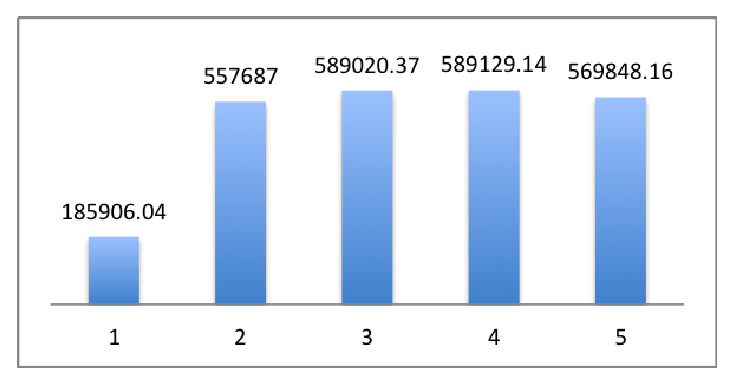
\includegraphics{perf_ngramlen1-5_distinct-items_supp10+_1hr.eps}}
\rput(18.89,0.5441601){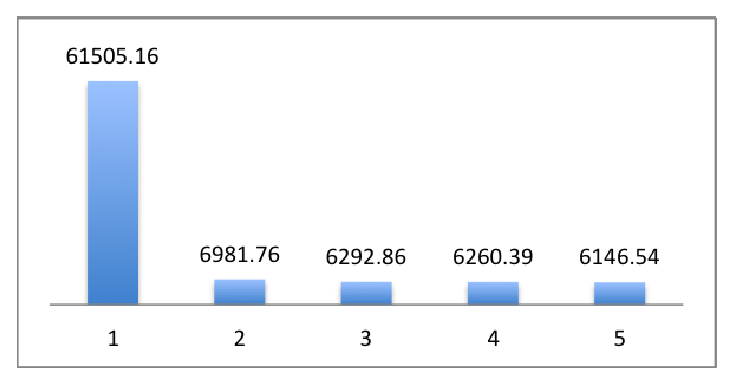
\includegraphics{perf_ngramlen1-5_itemsets_supp10+_1hr.eps}}
\rput(31.89,0.50416017){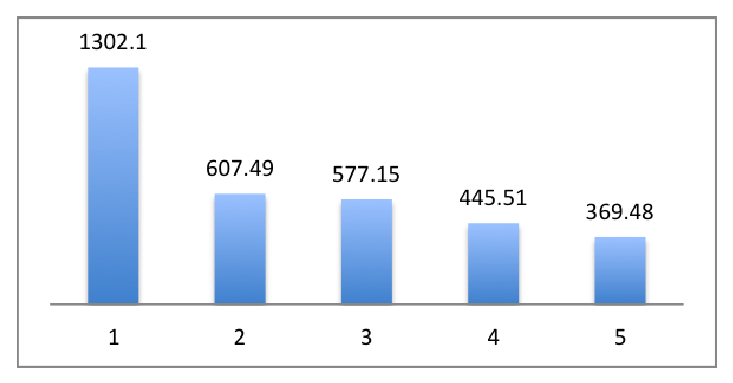
\includegraphics{perf_ngramlen1-5_runtime-millis_supp10+_1hr.eps}}
\end{pspicture} 
}
\caption{Effect of the increasing maximum N-Gram length on results of mining of 1hr epochs of data}
\label{fig:ngramsLen}
\end{figure*}

After mining term N-Grams we flatten the itemsets to sets of unigrams again. This removes overlap between parts of  itemsets making it easier to reason about how they relate to each other. 
%This also avoids the possibility that an itemset might be represented differently at different epochs. Actually, within one epoch 
This is also necessary since an itemset will have different N-Gram set representations, and its  postings list is the union of those of the different representations.
%, and its support would have been lost if not for maintaining the postings list. 
%We merge the union of the posting lists of all the N-Gram sets flattened to the same itemset.

%After flattening, we remove one more type of uninteresting itemsets produced just because the definition of closed itemsets cover it - the empty itemset and individual unigrams. In the rest of this paper we exclude them altogether, so an itemset  simply by not producing an itemset whose length is less than 2.


%\subsection{Choice of epoch span}
%\label{sec:span}
%Figure \ref{fig:numItemsetsVsSpan} shows the number of itemsets mined from different spans, using the same support threshold. The number of itemsets is higher when the span is shorter than 1 hour because the frequency required to surpass the support threshold  becomes very low (7 on average), and thus more noise itemsets are mined. The flat shape after the 1 hour mark shows that the itemsets mined from the shorter epoch spans are not included in the mining results of longer spans. Therefore, we will mine epochs of 1 hour span for the rest of the paper. 

%The numbers of both closed and maximal itemsets are shown, to give an intuition about the shape of the itemsets prefix tree. The small difference between the closed and maximal itemsets indicates that there is more breadth than than depth in the tree, since there aren't many internal nodes (closed itemsets that are not maximal). We discuss why this structure is formed and how to make use of this intuition in the following section.
%This is a good segway to what we will discuss 

%length of the epoch span used changes the nature of itemsets mined, . 
%\begin{figure}
%\centering
% Generated with LaTeXDraw 2.0.8
% Sat May 04 11:23:51 EDT 2013
% \usepackage[usenames,dvipsnames]{pstricks}
% \usepackage{epsfig}
% \usepackage{pst-grad} % For gradients
% \usepackage{pst-plot} % For axes
%\scalebox{1} % Change this value to rescale the drawing.
%{
%\begin{pspicture}(0,-2.74)(8.22,2.74)
%\rput(4.11,0.0){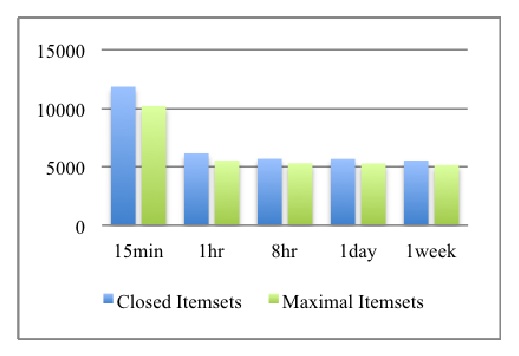
\includegraphics{mean-itemsets-count_change-with-epochlen_closed-maximal.eps}}
%\end{pspicture} 
%}
%\label{fig:numItemsetsVsSpan}
%\caption{Number of itemsets mined from different epoch spans, using N-Grams as items with N $\le$ 5} 
%\end{figure}


\section{Strengthening closure}
%Strongly closed itemsets}
\label{sec:strong}


\begin{figure}
\centering
% Generated with LaTeXDraw 2.0.8
% Thu May 09 12:02:46 EDT 2013
% \usepackage[usenames,dvipsnames]{pstricks}
% \usepackage{epsfig}
% \usepackage{pst-grad} % For gradients
% \usepackage{pst-plot} % For axes
\scalebox{0.9} % Change this value to rescale the drawing.
{
\begin{pspicture}(0,-2.649212)(9.077745,2.95)
\psframe[linewidth=0.04,dimen=outer](8.843161,2.95)(0.2431605,-2.61)
\usefont{T1}{ptm}{m}{n}
\rput(4.103317,1.675){sham, and, travesty}
\usefont{T1}{ptm}{m}{n}
\rput(1.7484828,2.575){@realdonaldtrump}
\pscircle[linewidth=0.04,dimen=outer](4.1031604,0.01){2.28}
\rput{55.644855}(2.9522903,-5.6005197){\psellipse[linewidth=0.04,dimen=outer](6.782275,-0.0031560312)(1.9103949,2.0626228)}
\rput{34.21703}(0.13301769,-1.7201583){\psellipse[linewidth=0.04,dimen=outer](2.8607624,-0.6440031)(2.908739,0.81)}
\pscircle[linewidth=0.04,dimen=outer](4.5031605,-0.33){1.58}
\usefont{T1}{ptm}{m}{n}
\rput(4.527965,-0.865){not,}
\pscircle[linewidth=0.04,linestyle=dashed,dash=0.16cm 0.16cm,dimen=outer](2.6031604,0.81){0.48}
\usefont{T1}{ptm}{m}{n}
\rput(1.0566566,1.455){fraud}
\pscircle[linewidth=0.04,linestyle=dashed,dash=0.16cm 0.16cm,dimen=outer](1.0631605,1.45){0.46}
\usefont{T1}{ptm}{m}{n}
\rput(2.623102,0.815){hair}
\pscircle[linewidth=0.04,dimen=outer](7.3231606,-1.35){1.02}
\usefont{T1}{ptm}{m}{n}
\rput(7.337262,-1.025){the, world, }
\usefont{T1}{ptm}{m}{n}
\rput(7.264635,-1.325){is, laughing}
\rput{34.21703}(0.8391447,-4.3701773){\psellipse[linewidth=0.04,dimen=outer](7.5185595,-0.8219682)(1.3607179,0.95923364)}
\rput{34.21703}(0.3818179,-4.274056){\psellipse[linewidth=0.04,dimen=outer](7.133755,-1.5167968)(1.2777647,0.86427283)}
\usefont{T1}{ptm}{m}{n}
\rput(7.207018,-1.645){at}
\usefont{T1}{ptm}{m}{n}
\rput(8.076705,-0.165){us}
\usefont{T1}{ptm}{m}{n}
\rput(6.371842,-2.105){you}
\usefont{T1}{ptm}{m}{n}
\rput(1.4102015,-1.625){elections}
\usefont{T1}{ptm}{m}{n}
\rput(6.9122915,1.255){rt}
\usefont{T1}{ptm}{m}{n}
\rput(4.4461293,-1.265){democracy}
\end{pspicture} 
}

\caption{Closed, distinct and strongly closed sets}
\label{fig:sham}
\end{figure}

The closed property of an itemset is easily violated by modifying one transaction that contains the itemset and removing one of its items. While an update operation is not supported in the model of frequent itemsets mining, a similar effect happens when people are writing about a certain fine grained topic. For example, figure \ref{fig:sham} illustrates  itemsets related to Donald Trump's famous 
%meltdown 
Tweets when Obama's victory was clear\footnote{http://www.huffingtonpost.com/2012/11/07/donald-trump-election-revolution\_n\_2085864.html}.  
Each area in the figure represents the transactions containing the itemset formed by concatenating the items in all intersecting ellipses.  

The figure shows the effect of the lack of context and structure in conversations happening on Twitter. Because there was originally no way to refer to a certain Tweet, a Tweet that sparks conversation on Twitter had  to be quoted in a retweet along with the retweeter's comment on it. This tradition still continues even though now Tweets can reference each other. 
%Because there was originally no way to refer to a certain Tweet, retweets (forwards) had to quote the Tweet being discussed, and this tradition still continues even though now Tweets reference each other. 
Due to the 140 characters length limit of Tweets the quotation usually has to be made as short as possible by selecting only the most discriminative words. 

In the figure, the most discriminative words are ``sham, and, travesty'' which are quoted along with Donal Trump's user name in most of the retweets. Other people choose to also include ``not, democracy'' and/or ``elections'', and in most of the cases the retweet indicator ``rt'' is added. 
This selection is an act of collaborative filtering, but it results in many trivially different subsets from the original Tweet. The additions of retweeters also form many different supersets of the of the original Tweet, and some additions represent opinions that are supported enough to be mined as itemsets. 

%Empirically, the difference between the number of closed itemsets and maximal itemsets of length 2 or more (i.e. excluding itemsets that are merely a frequent term) is rather small; the means across all hour long epochs in 
%Tweets posted in November 
%our data are 2439.17 closed itemsets and 1831.92 maximal itemsets. 



We propose two conditions that are not as easily violated as the closed condition for selecting itemsets. The two conditions build on the concept of \emph{association rule confidence}. Confidence is the basic property used for association rules mining, and it is used in the definition of $\delta$-free sets \cite{boulicaut2003free}. Mining itemsets based on the confidence of rules they induce has long been recognized as a method for finding ``interesting patterns'' \cite{cohen2001finding}, but since this property is not anti-monotone a variation has to be used (for example, \emph{all confidence} \cite{kim2004ccmine}).The confidence of an assocation rule that the presence of an itemset, $s_{j}$, implies the presence of another itemset, $s_i$, is  defined as:
\begin{equation}\label{eq:conf}conf(s_j \rightarrow s_i) = \frac{|T_{s_i} \cap T_{s_j}|}{|T_{s_j}|}\end{equation}


\subsection{strongly closed itemset}

To remove the redundancy in closed itemsets we merge similar ones into \emph{strongly closed} itemset clusters. The similarity of an itemset, $s_i$, with another itemset, $s_j$, is measured as the overlap of the \emph{transactions} containing both of them with the transactions containing $s_j$. That is, the confidence of the rule $conf(s_j \rightarrow s_i)$. An itemset is clustered with another itemset if one exists such that the confidence exceeds a similarity threshold, $\kappa$.
% (the indistinctiveness of $s_d$ from $s_c$).
%(thus $\kappa \in \, ]0, 0.5]$ which is the reasonable range). 
If more than one itemset satisfies this condition, the itemset is clustered with the one implying it with the highest confidence. Ties are broken in favour of longer itemsets, and if two itemsets tie in both confidence and length the tie is broken arbitrarily. When an itemset is clustered with an itemset which is already part of a cluster, the itemset is added to the existing cluster. Finally, the \emph{strongly closed} itemset is the 
%bag of items formed by taking the 
union of all cluster members, and its support is the size of the union of their postings lists. We define the  desired clustering  and the strongly closed itemset represented by each cluster as follows:
\begin{multline}\label{eq:strongClosedFormal}
\mathcal{R} = \{r: r = \bigcup{(s_i, s_j)}\; where\; s_i \in \mathcal{C} \, and \, s_j \in \mathcal{C} 
\\\,and\; \forall_{(s_i,s_j)} \, s_j = \textbf{argmax}_{s_k} conf(s_k \rightarrow s_i) \\\;and \;conf(s_j \rightarrow s_i) \ge  \kappa\}
\end{multline}
\begin{equation}S_l = \{w:\, w \in \bigcup_{s_i \in r_l}{s_i} \; where \; r_l \in \mathcal{R}\}\end{equation}


\subsection{Distinct itemsets}
Clustering closed itemsets into \emph{strongly closed} itemsets don't solve the problem of redundancy caused by trivial differences in the language used. Consider, for example, that it is possible to say that ``Obama was elected'' as well as ``Obama got elected''. 
%, resulting in different  itemsets because of a slight variation in the language. Note that 
Because of  the way PPC-Extension produces itemsets, 
%itemsets produced from the above sentences will be ordered according to the total ordering. 
and if the total ordering follows the descending order of items' frequencies, the itemsets generated will most likely be (in order and omitting 1-itemsets): \{was, obama\}, \{was, obama, elected\}, \{got, obama\}, \{got, obama, elected\} and \{obama, elected\}. The only itemset that carries a \emph{distinct} piece of information is \{obama, elected\}, and the rest is redundancy caused by slight variations in the language used.

We exploit the way PPC-Extension produces itemset when the total ordering follows the descending order of items' frequencies to define a condition for selecting \emph{distinct} itemsets. In this case, every itemset is generated by appending an item of lower frequency than items already in the itemset. The call tree of recursive LCM calls will be similar to an FP-tree. Given the length constraint on Tweets, then the tree can only be shallow and wide. Therefore, an itemset that has a large number of supersets cannot be the root of a tree with a limited number of deep branches, but it has to be covering a breadth of possible descendants. If the itemset does not imply any of its supersets with high confidence, then this itemset does not represent a \emph{distinctive} piece of information. For example, \{was, obama\} and \{got, obama\}  are not informative because \{was\} and \{got\} can appear with many other items, and they appear with most of them equally likely. On the other hand, if an itemset implies a superset with high confidence then this superset represents a \emph{distinctive} piece of information. For example, \{obama, elected\} is implied by \{obama\} with high confidence.

We define a \emph{distinct} itemset, $s_i$, as a closed itemset 
%whose frequency comprises more than a certain proportion of the frequency of its least frequent subset, $s_j$; that is, 
which can be implied from the subset, $s_j$, by a confidence more than a threshold, $\delta$. We choose to use a similar notation to the one used in the definition of $\delta$-free itemsets because the parameter represents the confidence of the rule ``$s_j \rightarrow s_i$'' in both cases. However, we filter out the subset so that the information in the superset is preserved, while in the case of $\delta$-free itemsets the supersets were filtered out.
%, or which has at least one strongly closed superset. 
%This condition chooses closed itemsets which substantially violate the closed condition of their subsets, which we interpret as being dissimilar from their subsets. Hence, we use the same similarity threshold, but instead of enforcing that $\kThe proportion is a parameter, , that controls the selectivity of the \emph{distinctiveness} condition. 
Formally, the set of \emph{distinct} itemsets, $\mathcal{D}$, is defined as follows:
%We state this condition formally as follows:
%Let $\kappa$ be a parameter that can vary between 0 and 1 to increase the selectivity of the condition. Then the set of  \emph{high confidence} itemsets is:
%\begin{equation}\mathcal{S} = \{s:\frac{|T_{s}|}{|T_{s_{parent}}|} \, where \, s_{parent} \subset s \, and \, |T_{s_{parent}}| < |T_{s_{ancestor}} | \forall s_{ancestor} \subset s \}\end{equation}
\begin{equation}\mathcal{D} = \{s: s \in \mathcal{C} \, and \, \exists \; s_{p} \subset s \; where \; \frac{|T_{s}|}{|T_{s_{p}}|} \ge \delta %\, and \, |T_{s_{p}}| < |T_{s_{a}} |\, \forall \, s_{a} \subset s 
\}\end{equation}

In the example of ``obama, elected'', the itemset \{got, obama\}  will not be \emph{distinct} since ``got'' appears in many other supersets and doesn't imply \{got, obama\} with high confidence. IEven if  The same for \{was, obama\},

%Also, regardless of the  the volume of posts about a topic, the number of itemsets representing it should be limited and only the most \emph{distinctive} ones. the importance of particular opinions represented by itemsets with 

We define a condition to filter out itemsets that are not \emph{distinct} from their subsets and supersets, 

We exploit the way PPC-Extension produces itemset to introduce an optimization that improves both runtime, memory requirements and filtering power of the high confidence condition. Unlike the original LCM algorithm, filtering low confidence itemsets requires keeping mining resluts in memory to calculate the confidence of newly generated ones.

%any of their subsets - notice that
%, and itemsets which are present in too many supersets.

Itemsets that are not \emph{distinct} from any of their subsets can be filtered out by setting a lower bound on the amount of transactions containing the subset but not the superset, specified as a ratio which we take to be $1 - \kappa$. This is equivalent to filtering out itemsets that are not implied by their subsets with confidence at least $1 - \kappa$. Examples of such itemsets are the ones in dashed lines in figure \ref{fig:sham}.

clustersdescribed can sho

The clustering scheme described selects the cluster that contains the itemset which maximizes the confidence of the rule $conf(s_c \rightarrow s_d)$, with a lower bound on the overlap to maintain distinctiveness. Formally, the clustering result are: 



We notice that itemsets related to each fine grained topic overlap with one another, forming a hierarchical cluster. In the figure there are two clusters about two Tweets that Donald Trump sent in the same hour. The retweet indicator joins the two clusters together, since it appears in itemsets pertaining to both Tweets. and any functional word can join any




\emph{distinct} itemsets, in solid lines, and closed itemsets that don't satisfy the distinctiveness condition, in dashed lines. %the circle with the words in its container. 
The figure represents
%The term ``rt'' indicates a retweet (forwarding a Tweet).
% Figure \ref{fig:sham} 


 on November 6th, 2012 many people where tweeting that ``(\underline{Barack} Obama) was elected (\underline{as president \underline{of the United States \underline{of America}}})''. If all the Tweets which use the verb phrase ``was elected'' to report the event also contain the two names (in parenthesis) in full, then there will be one  \emph{maximal}  itemset with all 12 items. However, either or both the names can be shortened by omitting an underlined part and still convey the meaning. 
%We can consider Tweets with any combination of shortened names to be modifications of the \emph{maximal} closed itemset. 
Therefore instead of 1 maximal itemset about the event there will be 8 closed ones. Nevertheless, mining only \emph{maximal} itemsets doesn't solve the problem of redundancy. Consider that it is possible to say that ``Obama was elected'' as well as ``Obama got elected'', resulting in 2 maximal itemsets because of a slight variation in the language. Empirically, this is evident in the relatively small difference between the number of closed itemsets and maximal itemsets of length 2 or more (i.e. excluding itemsets that are merely a frequent term); the means across all hour long epochs in 
%Tweets posted in November 
our data are 2439.17 closed itemsets and 1831.92 maximal itemsets. 


%For example, on November 9th, 2012 many people where tweeting that ``Justin Bieber and Selena Gomez broke up''. If all Tweets which use the verb "break up" to report the topic also contain the two names in full, then there will be one closed itemset with all 6 items. However, a Tweet can contain any of 8 other combinations of the four names that fully convey the meaning. We can consider that Tweets with any of these combinations are modifications of the \emph{maximal} closed itemset. Therefore instead of 1 maximal itemset about the topic there will be 9 closed ones. Now consider that it is possible to say that "Justin and Selena broke up" as well as "Justin broke up with Selena", resulting in 2 maximal itemsets. This increase in the number of maximal itemsets because of slight variations in the language is intensified by the length limit on Tweets, specially when people try to make space for their comment about a Tweet they are retweeting. We therefore need a property between the easily violated closed property and the very strict maximal property which also results in a large number of redundant itemsets. 
% This will result in the creation of two closed itemsets, a new shorter with support that one higher than the original itemset
Trivial violations of the closure condition can be filtered out by setting a lower bound on the amount of transactions containing the subset but not the superset, specified as a ratio $\kappa$. This is equivalent to filtering out itemsets that are not part of any rule with confidence at least $\kappa$. However, this condition is met by many language constructs, and \emph{even though} the superset occurs in a substantial proportion of the transactions containing the subset they are not distinctive from each other, but rather expected to appear together - notice that we had to flatten N-grams itemsets back to unigram itemsets. 

Given the length constraint on Tweets, then the 
%FP-Tree can only be shallow and wide. 
size of itemsets will also be limited. Therefore, an itemset that has a large number of supersets cannot be appearing with only a limited set of words (topic), but it has to be covering a breadth of possible descendants. Thus this itemset is very likely to be a language construct. Even if it is a language construct that appears with high confidence with some topical words 
%, this high confidence doesn't carry interesting information; for example, \{the, of\} that appears within \{the, united, states, of, america\}. Even if it is a 
or is an itemset made up topical word with very high frequency, then interesting information will be divided into several subtopics given its large number of direct descendants. In either case, filtering closed itemsets implied with high confidence by such a ubiquitous itemset will not omit any information. Any set of items that convey specific information will be part of an itemset whose longest subset is not part of many other supersets.
%If the filtered itemset is part of an informative one then it will be produced as part of the longer itemset 
%is found to have high confidence with the filtered one.

We exploit the way PPC-Extension produces itemsets to filter out collocations that are language constructs and select only meaningful ones. If the total ordering of items follows the descending order of items' frequencies, then the call tree of recursive LCM calls will be very similar to the FP-tree.  

%to introduce an optimization that improves both runtime, memory requirements and filtering power of the high confidence condition. Unlike the original LCM algorithm, filtering low confidence itemsets requires keeping mining resluts in memory to calculate the confidence of newly generated ones.
% forming strong closed clusters requires keeping itemsets in memory so that newly generated ones are clustered with them.
% to find candidates for merging. 
Instead of keeping all previous itemsets in memory we keep only a limited number, $b$ (for buffer size). This obviously improves runtime and memory requirements, and it can also improve the choice of itemsets. I
%For a large enough $b$, 
%if an itemset is produced $b$ steps ago then this itemset's overlap with the current itemset is very likely a language construct. Since the tree is shallow, then 


We use a buffer size $b=1000$ in all experiments, which leads to a runtime of about 1 to 3 milliseconds per itemset for filtering out low confidence itemsets and creating strong closed clusters. The number of selected itemsets is also reduced by almost half on average. The difference between the two selections is made up mostly of stop words. A few itemsets including topical words are also filtered, such as the closed itemset \{president, Obama\} since Obama is an example of a ubiquitous topical word. Such itemsets lack any information on their own and is included in other informative ones. Finally, this enhancement is not necessary for satisfactory performance. With an unlimited buffer, the average runtime is 5.2 seconds for filtering 4265 itemsets (the average number of closed itemsets from an hour long epoch)

%It also filters out itemsets that are short language constructs, because their components appear very frequently and none of their numerous supersets comprise a significant proportion of their high frequency. 





This clustering can be implemented efficiently using techniques similar to the ones proposed by Bayardo et al. \cite{bayardo2007scaling}. The main ideas are to limit the comparisons to a few candidates, and to terminate the comparison early if the similarity threshold will not be met. In our case the postings lists are longer than the itemsets, so we generate candidates for comparison by calculating similarity between itemsets. When calculating the similarity between two postings lists, we can terminate early if the difference exceeds the 
%value given by equation \ref{eq:maxDiffCnt}, which is derived from equation \ref{eq:conf}. It gives the 
maximum difference permissible to achieve a similarity of $1-\kappa$, which can be easily derived from equation \ref{eq:conf}. 
%From equation  \ref{eq:conf} the maximum difference between the transactions containing the antecedent of a rule and their intersection with those containing the consequent, is $\Delta$.
%those containing both the antecedent and the consequent 
%so that the confidence exceeds a threshold $proportion$. 
%the maximum difference allowed between the transactions containing the antecedent of a rule and those containing both the antecedent and the consequent so that the confidence exceeds the distinctiveness threshold $\kappa$. It is easily derived from equation \ref{eq:conf}.

%\begin{equation}\label{eq:maxDiffCnt}\Delta(s_{antecedent},  proportion)
%similarity = (1 - \kappa)) 
%\le proportion *  |T_{s_{antecedent}}|
%\end{equation}

Algorithm  \ref{algo:alliance}  shows a possible implementation. For each itemset, $s_i$, we find the itemsets produced before it and overlapping with it in one or more item. Out of those candidates, $s_c$, we find the one that maximizes $conf(s_c \rightarrow s_i)$ such that the confidence exceeds $1-\kappa$.
%such that the \emph{similarity} condition holds - that is, the \emph{distinctiveness} condition \emph{doesn't} hold. 
Notice that confidence is not a symmetric measure, and we only check the confidence of the rule that the clustering candidate implies the itemset. 
% but it is only meaningful to check the confidence of the rule from 
%the higher support shorter itemset to the lower support longer itemset. Higher support shorter itemsets will be produced before the itemset being clustered because of the way PPO-Extension produces itemsets, when the total ordering follows the descending order of items' frequency. 
%The functions difference() terminates early, and it also doesn't need to traverse the postings lists at all when calculating the difference between an itemset and one of its subsets. In this case the size of the difference will be $|T_{s_c}| - |T_{s_i}|$.


\begin{figure}
% Generated with LaTeXDraw 2.0.8
% Sat May 11 09:28:32 EDT 2013
% \usepackage[usenames,dvipsnames]{pstricks}
% \usepackage{epsfig}
% \usepackage{pst-grad} % For gradients
% \usepackage{pst-plot} % For axes
\scalebox{.5} % Change this value to rescale the drawing.
{
\begin{pspicture}(0,-4.16)(16.6,4.16)
\rput(8.3,0.0){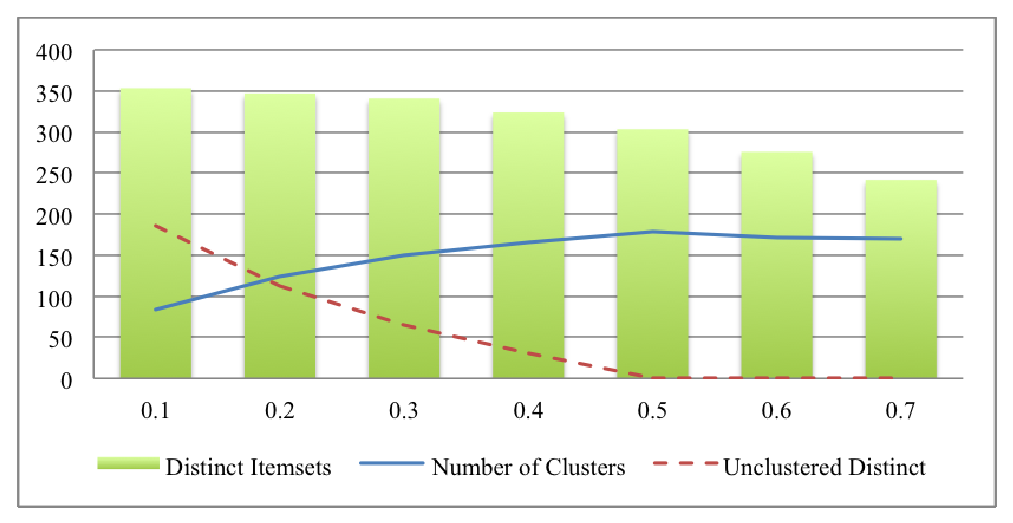
\includegraphics{kappa_effect.eps}}
\end{pspicture} 
}
\caption{Effect of changing $\kappa$ on mining results }
\label{fig:kappa}
\end{figure}


\begin{algorithm}
\SetAlgoLined
\LinesNumbered
\KwIn{$\kappa$: Minimum distinctiveness threshold} % closed strength} %$\theta$: Minimum cosine similarity, \\
\KwData{$\mathcal{C}$: Closed Itemsets produced by LCM}
\KwResult{$\mathcal{R}$: Strong closed itemset clusters}
\For{$i \gets 2$ to $|\mathcal{C}|$}{
	$C \gets \{s_c: s_c \in \mathcal{C} \, and \, c < i \, and \, |s_c \cap s_i| > 0\}$\;
	$P \gets \{s_p: s_p \in \mathcal{C} \, and \, p < i \, and \, s_p \cap s_i = s_i\}$\;
	$s_p \gets \textbf{argmax}_{s_p \in P}\frac{|T_{s_i}|}{|T_{s_p}|}$ \tcp*{Direct parent}
	\uIf{$\frac{|T_{s_i}|}{|T_{s_p}|} < \kappa$}{continue\tcp*{Not a distinct itemset}}
	$s_m \gets s_i$  \tcp*{Cluster centroid, initially self}
	$maxConf \gets 0$ \tcp*{Best candidate's score}
	\ForEach{$s_c \in C$}{
		$\Delta \gets (1 - (1-\kappa)) |T_{s_c}|$ \tcp*{Maximum difference}
		$\delta \gets$ difference($T_{s_c},T_{s_c \cup s_i},\Delta$) \tcp*{Stops early}
		
		\If{$\delta \le \Delta$}{ %and $\delta < minDiff$}{
			$conf \gets \frac{|T_{s_c}| - \delta}{ |T_{s_c}|}$\;
			\If{$conf > maxConf$}{
				$s_m \gets s_k$ \tcp*{Best merge candidate}
				$maxConf \gets conf$ \;%\delta$\; 
			}
		}
	}
	$\mathcal{R}[s_i] \gets \mathcal{R}[s_m]$ \tcp*{Cluster $s_i$ with $s_m$}
	$\mathcal{R}[s_m].itemset \gets \mathcal{R}[s_m].itemset \cup s_i \cup s_m$\;
	$\mathcal{R}[s_m].postingsList \gets \mathcal{R}[s_m].postingsList \cup s_i.postingsList \cup s_m.postingsList$\;
}
\Return{$\mathcal{R}$}\;
\caption{Forming strong closed itemset clusters}
\label{algo:alliance}
\end{algorithm}

Figure \ref{fig:kappa} show the effect of varying $\kappa$ on the mean number of \emph{distinct} and \emph{strong closed} itemsets mined from 1 hour long epochs. The number of \emph{distinct} itemsets keeps dropping as the distinctiveness threshold increases. On the other hand, the number of \emph{strong closed} clusters formed keeps increasing as the similarity (indistinctiveness) threshold decreases. The dashed line shows that the number of unclustered distinct itemsets reaches zero at $\kappa=0.5$, which explains why the number of clusters changes very slightly after that. 
%This indicates that it is unlikely that impure clusters are formed even though the similarity threshold is low. 
We use $\kappa = 0.25$ for the rest of the paper, which is an arbitrary choice based on the definition not the data. The average number of itemsets (\emph{strongly closed} and unclustered \emph{distinct}) mined from 1 hour epochs at this value of $\kappa$ is only 224.48 which is about 10\% of the number of closed itemsets.
% (2439.17).
%of length 2 or more.
%and any other positive number less than 0.5 can be used. 
%If a distinctiveness threshold of 0.5 or more is desired then the similarity threshold ought to be explicitly set, because a similarity of 0.5 or less may result in impure clusters. 


%After joining an alliance an itemset seizes to exist outside of the alliance, so that an itemset can be part of only one alliance. However, when checking which itemsets to consider for merging with a still unallied itemset, its similarity is calculated with the individual itemsets rather than the alliance. Otherwise, an itemset could fail to join an existing alliance because the similarity between the larger bag of items and the itemset is likely to be lower than the similarity between individual member itemsets and the itemset. This can cause cascading many alliances that should have been separate into one large alliance. Such an oversized alliance could also be about different topics. Empirically, we observe that one and only one oversized alliance about different topics is formed. This alliance catches many itemsets made up of low IDF terms, thus not interesting. Topics with high IDF terms in them cannot have high cosine similarity with topics of only low IDF terms. The size of the bag of items in this alliance is significantly larger than other alliances, making it easy to distinguish and discard it.
%It is difficult to reason about how alliances are formed, specially after fi

%Expanding on the previous observation that adding a high IDF term to an itemset with low IDF terms only prevents achieving a high enough cosine similarity, we introduce an optimization that improves both runtime, memory requirements and filtering power. Unlike the original LCM algorithm, our extension requires keeping previous itemsets in memory so that newly generated ones are compared to them to find candidates for alliance. Instead of keeping all previous itemsets in memory we keep only a limited number, $b$. This obviously improves runtime and memory requirements, but it also improves the quality of itemsets chosen for alliance. Given the way PPC-Extension produces itemsets, an alliance candidate appearing more than $b$ itemsets earlier must be similar because of a term that has at least $\log_2(b+1)$  extension items \emph{smaller} than the one that got added to form the current itemset. This lower bound assumes that all possible itemsets created by appending any combination of the $\log_2(b+1)$ will be closed and will have enough support. In this case, there will be 1 combination where all the items are appended, $\log_2(b+1)$ combinations where one item is missing, $\log_2(b+1)$ choose 2 combinations where 2 items are missing, ... etc. For all of these combinations to be closed itemsets, the 1 combination where all the items are appended has to have minimum support, the  $\log_2(b+1)$ combinations where 1 item is missing will each have support 1 more than minimum, the combinations where 2 items are missing will each have support 2 more than minimum, ... etc. Therefore the minimum drop in frequency between a closed itemsets and its subset produced $b$ steps earlier is given by:
%\begin{equation}|D_{S_x}| - |D_{S_(x-b)}| = \alpha \frac{|E|}{E.span} + \sum_{a=1}^{\log_2(b+1) - 1}a\binom{\log_2(b+1)}{a} \end{equation}
%To minimize the difference in frequency between the current itemset and the alliance candidate, we assume that the 1 combination will appear $\ciel{b/2}$ times,  Therefore the difference in frequency between  $b$ 

%A similar situation also happens if the intersection ???
%must have a frequency of occurrence at least $b$ more than the current itemset's frequency. 

%Algorithm \ref{algo:alliance} shows the described algorithm for merging itemsets alliances. Table  \ref{table:allianceQuality} shows the number of closed itemsets of length at least 2 without filtering any of them out, as well as after applying the KLD filter and the strongly closed filter, and the number of itemsets alliances. The table also shows the average quality of the itemsets after each stage of reduction. The quality is calculated as Basic Elements? PERPLEXITY? CASCADE MEASURE? 

\subsection{Bounding runtime and memory}
\label{sec:bounding}
%Expanding on the previous observation that adding a high IDF term to an itemset with low IDF terms only prevents achieving a high enough cosine similarity, 
.

Figure \ref{fig:lcmvsfpzhu} shows the total runtime of the LCM algorithm plus the strong closed itemsets clustering (LCM + Clustering) at different epoch spans. The runtime of LCM alone is also plotted for reference. We also plot the performance of another frequent itemset mining algorithm, FP-Zhu \cite{grahne2004reducing}, which was the runner up at FIMI '04   \cite{DBLP:conf/fimi/2004}. We include it to show that our extensions do not degrade the performance of LCM even in the context of competitions. The Y-Axis is in logarithmic scale to keep the scale of the plot suitable for seeing slight differences. The output of LCM is the input to the clustering algorithm, so it is affected by the number of closed itemsets produced. This explains why it takes slightly longer time for clustering results from the 15 minutes epoch and then takes a constant time for epochs of longer span.

\begin{figure}
\centering
% Generated with LaTeXDraw 2.0.8
% Sat May 11 10:40:24 EDT 2013
% \usepackage[usenames,dvipsnames]{pstricks}
% \usepackage{epsfig}
% \usepackage{pst-grad} % For gradients
% \usepackage{pst-plot} % For axes
\scalebox{0.6} % Change this value to rescale the drawing.
{
\begin{pspicture}(0,-4.52)(16.408476,4.52)
\rput(7.52,0.0){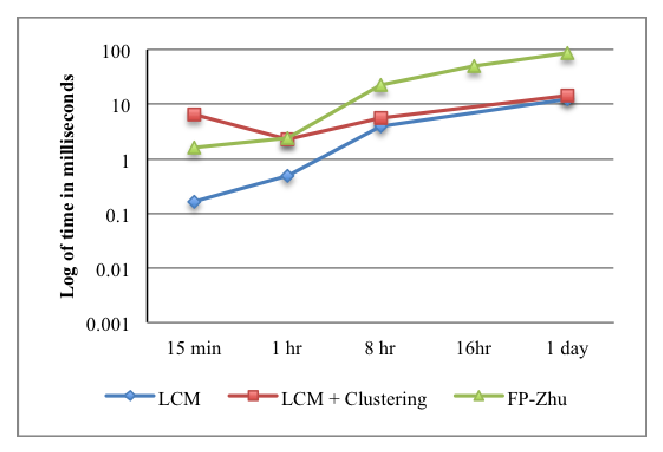
\includegraphics{/Users/yia/Code/thesis/write-ups/cikm/runtime_lcm-lcm+filter-fpzhu_seconds.eps}}
\usefont{T1}{ptm}{m}{n}
\rput(14.1,-3.85){\large ($\kappa = 0.25$)}
\end{pspicture} 
}
\caption{Runtime of itemset mining alone and with filtering and clustering at different epoch spans}
\label{fig:lcmvsfpzhu}
\end{figure}
% select args, count(*), avg(value), stddev(value) from perf_mon where args like '%oct-nov-dec/%Jaccard+_%ULBuff%' and key = 'CPUMillisFilter' group by args order by args;
 
%Furthermore, the clustering is improved for some itemsets because of filtering noisy ones. For example, ``ballot''
%only be a very frequent set of items. The number
%, because of the way PPC-Extension produces itemsets, for an itemset $S_x$ and any candidate subset $S_{(x-b)}$ that was produced $b$ itemsets earlier $|D_{S_{(x-b)}}| - |D_{S_x}| \ge b$. This lower bound is achieved when the intersection of the documents containing the current itemset $S_x$ and all the $b-1$ supersets before it is exactly the subset $S_{(x-b)}$, and there are no more itemsets with the same intersection. In this case each of the $b$ supersets must have support at most $|D_{S_{(x-b)}}| - 1$ to be considered closed, but because there are $b$ of them then actually their support is $|D_{S_{(x-b)}}| - b$. Since the minimum support difference is $b$, then the maximum confidence of $S_x$ is $\frac{|D_{S_{(x-b)}}| - b}{|D_{S_{(x-b)}}|} $. Therefore for a given $\kappa$ we can determine the buffer size $b$ as the frequency of itemsets keeps decreasing. In our implementation we use a fixed $b$ of 1000.


% The difference between documents containing a certain strongly closed itemset and the intersection can be as little as one document. Thus all variations can have high confidence. On the other hand, using an upper bound on confidence is totally counter intuitive, since this means that if only one document exists with a shorter itemset then the longer itemset will be omitted. 
%Observe that all documents containing the longer itemset will also contain the shorter itemset, and it is possible for several variations to have high confidence because documents
%filters out many redundant closed itemsets, but cannot filter out formed because of slight variations of the same topic. 

%We build on the confidence property by merging high confidence itemsets that are extensions of the same itemset into an itemset \emph{alliance}. The itemset alliance is a bag of items formed by taking the union of all member itemsets. This concentrates the numerous high confidence closed and maximal itemsets about a certain topic into one unit. Furthermore, we also include in the alliance all itemsets with high cosine similarity to its members. This merges together itemsets that differ because of items that come earlier in the total ordering and are not pertaining to the topic, such as ``with'' and ``and'' in the Bieber-Gomez example. To avoid forming alliances that are not coherent about a certain topic, we go beyond the numerical calculation of confidence and we actually calculate the overlap between the posting lists of itemsets being merged. In case of merging an itemset with its subset 
%With a reasonably high support, the 
%\subsection{Effect of confidence threshold}%Choice of $\kappa$}
%Figure \ref{fig:numStrongHConf} shows the number of high confidence itemsets (of length more than 1) at different values of $\kappa$. Even at low values of $\kappa$, the number is much lower than the number of closed itemsets (6147 from figure \ref{fig:ngramsLen}, but only 2440 after removing 1-itemsets). This encourages us to use a low value of $\kappa$, since the biggest reduction in number of itemset has already happened by filtering out itemsets that don't make up any significant proportion of their subsets'  support. We use $\kappa=0.2$ for the rest of the paper. 

%The number of strong closed itemset clusters, and its ratio to the number of high confidence itemsets are also shown. While the number of high confidence itemsets decrease as $\alpha$ increases, the ratio stays almost fixed. This indicates that regardless of the selectivity of the high confidence condition (or any other condition used) there will always be itemsets that can be clustered together, stressing the effect of language use. At $\kappa=0.2$, we are left with ~10\% of the closed itemsets of length 2 or more. The next two sections will show how to make sense of them.
%the selectivity of strong closed itemset clusters is $~\frac{200}/{2440}

%\begin{figure}
% Generated with LaTeXDraw 2.0.8
% Sun May 05 22:12:01 EDT 2013
% \usepackage[usenames,dvipsnames]{pstricks}
% \usepackage{epsfig}
% \usepackage{pst-grad} % For gradients
% \usepackage{pst-plot} % For axes
%\scalebox{0.5} % Change this value to rescale the drawing.
%{
%\begin{pspicture}(0,-5.37)(16.96,5.37)
%\rput(8.48,0.0){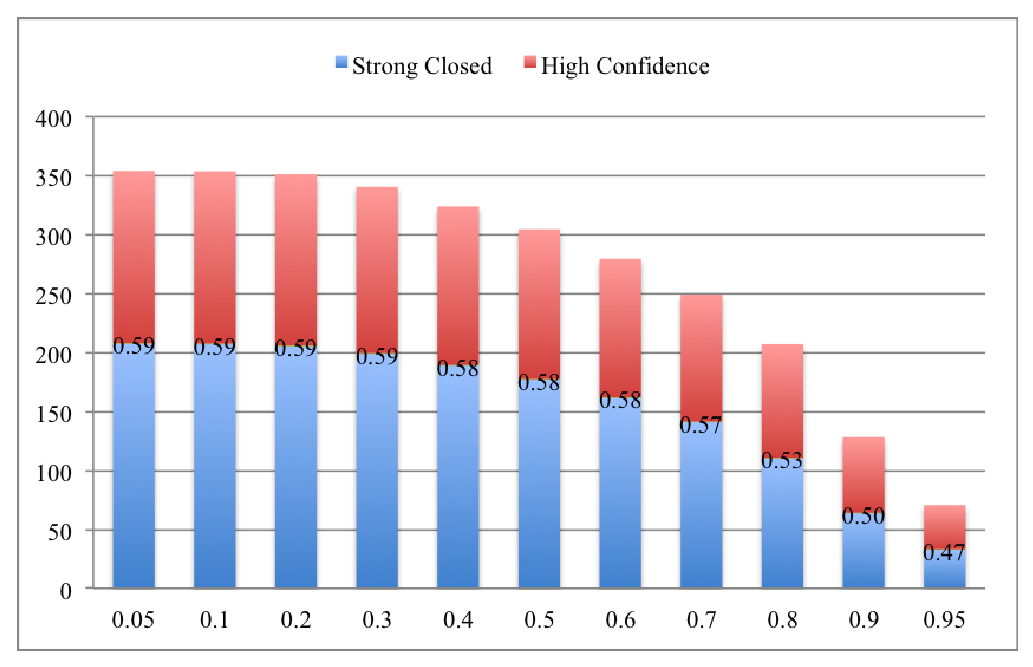
\includegraphics{num-itemsets_high-conf+strong-closed_against-kappa.eps}}
%\end{pspicture} 
%}
%\label{fig:numStrongHConf}
%\caption{Number of strong closed itemsets and high confidence itemsets at different values of $\kappa$}
%. The ratio of the two numbers is shown on top of the bar}
%\end{figure}

\section{Temporal Ranking}
\label{sec:rank}
%So far we have been reducing the number of itemsets, and we succeeded to reduce it to about 1\% of the original number (in alliances). We now discuss how to rank the itemset alliances, making use of the structure of the alliance. 
%We have experimented with various ranking schemes applied directly to itemsets (before and after reduction) and none of them resulted in a satisfactory ranking. 
%We exploit temporal features for ranking itemsets. exploit t
For ranking itemsets according to the importance of each itemset in within the mined epoch, we use itemsets' pointwise KL Divergence from a background model. The pointwise KLD of the probability of an itemset $s_i$ in the background model $Q$ from its probability in the current epoch $P$ can be considered the information gain, IG: 
\begin{multline}IG(P(s_i),Q(s_i))  = - (H(P(s_i)) - H(P(s_i),Q(s_i))) \\ = \sum{P(s_i) \log{P(s_i)}} - \sum{P(s_i) \log{Q(s_i)}}  = KLD(P(s_i)||Q(s_i))\end{multline}

To generalized this to the case of strong closed itemset clusters, we have to take the overlap between the itemsets of the cluster into account when calculating the information gain of the whole cluster.
We note that the joint probability of the itemset, $s_i$, and its superset, $s_j$, is equal to the probability of the superset; $P(s_i,s_j) = P(s_j)$ and $Q(s_i,s_j) = Q(s_j)$. 
Thus, the information gain of the appearance of an itemset and its superset together is essentially the information gain of the superset; $IG(P(s_i,s_j),Q(s_i,s_j)) = IG(P(s_j),Q(s_j))$.  Also, their Pointwise Mutual Information is the Self Information of the subset:
\begin{multline}
PMI(s_i, s_j) = \log{ \frac{P(s_i,s_j)}{P(s_i)P(s_j)} } = -\log{P(s_i)} = I(s_i)
\end{multline}

Therefore, the information gain of a superset is different from the information gain of its subset by the information gained (or lost) because of the additional items. Thus, the information gain of the appearance of all itemsets in a strong closed itemset cluster, $S=\{s_i1,..,s_im\}$, 
%an alliance of $m$ itemets, $S_{i1},S_{i2},...S_{im}$, 
can be calculated as the information gain of its smallest subset, $s_{min}$, plus the differences between the KLDs of member subsets and the smallest subset. We use the squares of the differences, because the pointwise KLD value can be positive or negative and we only care about the magnitude of the difference
%, depending on whether the subset appears with lower or higher probability than the background. 
To give the self information of the smallest subset the same influence, we also square it. Thus the information gain of a strong closed itemset is given by:
\begin{multline*}IG^2(P(s_{i1},...s_{im}),Q(s_{i1},...s_{im})) = I^2(s_{min}) + \\ %S_{i2},
\sum_{j = i1..im}{(KLD(P(s_j)||Q(s_j)) - KLD(P(s_{min})||Q(s_{min})))^{2}} \end{multline*}
%the squares of
%The difference is squared because the difference in information gain can be negative, however the information content is positive:
%can be explained in terms of mutual information. It is the mutual information between the itemset's appearance in  and 
%structure of the alliance produced by PPC-Extension if the total ordering follows the descending order of items' frequencies.

The formula above can be used directly for ranking clusters, but it will favour largers one.We normalize by the size of the cluster giving our final ranking formula for strong closed itemsets:
%the average information gain of an itemset in an alliance is give by:
\begin{equation}\label{eq:avgIG}\overline{IG}(S) = \frac{IG^2(P(s_{i1},...s_{im}),Q(s_{i1},...s_{im}))}{m}\end{equation}

%The ranking of strong closed itemsets according to equation \ref{eq:avgIG} gives superior results to many other ranking schemes we tried, including ones based on scores derived from the itemset content directly. 

%An intuitive explanation is that this ranking scheme gives high scores to clusters made up of a minimum set with small KLD and supersets with large KLD. According to the structure of the alliance produced by PPC-Extension if the total ordering follows the descending order of items' frequencies, the small KLD minimum subset will be an entity with sustained interest, and the high KLD supersets will be new appearing with probabilities very different from their background probabilities. In the next section we show the results of applying this ranking scheme along with the methods described in previous sections.

\subsection{Empirical Evaluation}
\label{sec:empirical}
%We have shown in the last 3 sections how to improve the efficiency of Frequent Itemsets Mining on social media data, by reducing the number of itemsets produced. To show the performance of the proposed methods in 
%filtering out itemsets that are uninteresting and 
%choosing important itemsets, we apply them on Tweets posted on the $6^{th}$ and $9^{th}$ of November 2012. In tables \ref{table:nov6} and \ref{table:nov9} we show the results of mining overlapping 1 hour epochs. Because of space limitation we show only the top 3 itemsets, ranked as described in section \ref{sec:allianceRank}, for each hour.
For the lack of ground truth data, the performance of the ranking (and the quality of the filtering and clustering on which it is based) is shown by example. The background model we use is the results of mining the previous month, using a \emph{minimum support} value of 1 occurrence (in the least volume hour). Mining the background model at such a low support increases the number of produced itemsets, which is desirable for a background model. All probabilities are smoothed by add-one smoothing. 

Tables \ref{table:nov6} and \ref{table:nov9}  show the top 3 itemsets for 1 hour epochs in the days of November 6th and 9th. The itemsets shown are the first appearances of the most interesting itemsets; that is, an hour is shown only if its top 3 feature novel interesting itemsets. The first column is the beginning of the hour, EST time. The second column is the top itemsets. The third column is a commentary to explain the itemsets, but we omit it from table \ref{table:nov9} to save space since the itemsets are self explanatory.
%, only for space limitation. The rest of the itemsets contain other formulations of the same pieces of news. An omitted hour doesn't  omitted hours either don't contain interesting news or conti.
%by point wise KL-Divergence against the results of mining the month of October. 

On November $6^{th}$, the US presidential elections took place and we can see how its events unwind from ``get out and vote'' to the projections and debates, all the way to the ``acceptance speech''. Early in the day, itemsets about UEFA Champions football matches and a TV show appear in the top 3 along with itemsets about the still uneventful elections. Actually, the matches keep occupying top positions and timely updates of their scores appear in the top 30 itemsets, until they end and the elections heats up. Short after the results of the elections became clear, news that ``weed is legal in Colorado'' occupies the top position. This exemplifies the power of social media as a collaborative filter, picking the important news even if it is unexpected. The user centric definition of importance is eminent in  the great attention given to the ``lady behind Obama  with a flag in her hair'' during the acceptance speech. 
% Throughout the day itemsets about the elections as well as about other topics are ranked high, even if they are topics in a language other than English and thus with a smaller supporting user base (such as the topic in Portuguese about when to consider a person old [velho]).
%UEFA Champions football games! We can 

On November $9^{th}$, no major events were happening but many overlapping minor ones happened. The day starts by news about the end of two careers; the Laker's ``coach Mike Brown'' got fired  and ``CIA director David Petraeus resigns''. The relationship of Justin Bieber also ends as he ``broke, up, with, Selena, Gomez'' at 22:00. This overlaps with his participation in the MTV Europe Music Awards (MTVEMA), and both topics occupied high rankings. MTVEMA is particularly interesting because votes were solicited from audience through Twitter. This is an example of a topic where people have different opinions, as the hour 15:00 shows. The top 3 itemsets of this hour are supporting ``Katy  Perry'', ``Justin Bieber'' and ``Lady Gaga'' respectively. They are all reported as separate itemsets, showing how clustering using the postings lists avoid forming incohesive clusters.
%The neutral itemset only soliciting votes is also mined and appears in the top 3 of other hours. 
By the end of the day many congratulations for the Indonesian Hero's day (``Hari Pahlawan'') appear, and the Turkish commemoration day of Ataturk is also mentioned as the 10th of November starts in these countries. These are examples of itemsets from languages with a relatively low number of users, showing how the absolute popularity of a topic doesn't affect its rank. If itemsets from only a specific language is desired, language identification can be applies on the itemsets and Tweets from their postings lists. Moving language identification downstream avoids affecting the results of mining because of error in an upstream component.

% (we refer to it as the \emph{MTVEMA voting invitation} to save space).
%To start off, the Laker's ``coach Mike Brown'' got fired and it was expected that either ``Phil Jackson [or] Jerry Sloan'' will succeed him. Another career end gets attention as ``CIA director David Petraeus resigns'', and an The MTV Europe Music Awards (MTVEMA) was also taking place and he also broke up with Selena Gomez. Therefore, this period contains events of different types that overlap, and we can use it to assess the effectiveness of our methods without access to ground truth data. The itemset alliances shown are the top 10 per hour ranked by point wise KL-Divergence against the results of mining the month of October. 
\begin{table}

\begin{center}
\small
\def\arraystretch{1.1}
\begin{tabular}{|p{.6cm}|p{2.5cm}|p{5cm}|}

\hline
\multirow{3}{*}{\texttt{13:00}} 	&  0, 1, de, jong 			& De Jong scores for Ajax \\ \cline{2-3} %http://www.dailymail.co.uk/sport/football/article-2228815/Manchester-City-2-Ajax-2--match-report-Siem-Jong-Yaya-Toure-Sergio-Aguero-Champions-League.html
					   	& geordie, shore		& Season 5 of the TV series starts \\ \cline{2-3}
						& get, out, and, vote		& Still early in the U.S. elections day \\\hline

\multirow{3}{*}{\texttt{17:00}} 	&  if, obama, wins		& Speculations regarding elections \\ \cline{2-3}
					   	& USERNAME, spots, my, club		&  Pyramidal marketing scam. Retweeted by people to make money.  \\ \cline{2-3}
						& the, polls, close		& Polls to start closing at 6 PM \\\hline %http://www.huffingtonpost.com/2012/11/06/what-time-do-polls-close_n_2080894.html

\multirow{3}{*}{\texttt{19:00}} 	&  A partir de que idade voc\^{e} considera algu\'{e}m velho?		& Internet meme from Brazil, discussing when to start considering a person old. \\ \cline{2-3}
					   	& food, stamps		& Discussions pertaining to elections \\ \cline{2-3}
						& linda, mcmahon, senate		&  Linda McMahon loses CT senate race \\\hline

\multirow{3}{*}{\texttt{20:00}} 	& obama, got, this		&  Announcing states that Obama got \\ \cline{2-3}
					   	& projected, winner		& Early projections about who will win \\ \cline{2-3}
						& moving, to, canada		&  Reaction to projections \\\hline


\multirow{3}{*}{\texttt{21:00}} 	& elizabeth, warren		&  MA senate elections winner \\ \cline{2-3}
					   	& popular, vote		& Comparing Popular vs Electoral votes \\ \cline{2-3}
						& who, is, the, president?		&  Anticipation for the elections results\\\hline
						

\multirow{3}{*}{\texttt{22:00}} 	& \#forward, \#obama2012		&  Obama won, time to move \#forward \\ \cline{2-3}
					   	& my, president, is, still		& Some were saying Black (skin colour), others Blue (party colour) \\ \cline{2-3}
						& back, in, office		&   Obama is back in office\\\hline

\multirow{3}{*}{\texttt{22:30}} 	& once, you, go, black		& A popular cultural reference.\\ \cline{2-3} %  .. you never go back. 
					   	& @realdonaldtrump, this, elections, ... [his famous Tweet] 		& Donald Trump is a Republican and he couldn't accept Obama's victory\\ \cline{2-3}
						& concession, speech, write		&   The losing candidate has to concede before the winner declares victory \\\hline
						
\multirow{3}{*}{\texttt{23:00}} 	& weed, is, legal, in, colorado		&  This piece of news got the attention as soon as it was announced  \\ \cline{2-3}
					   	& karl, rove		& Fox news challenges results from Ohio\\ \cline{2-3}
						& our, country, is, trouble		&   Dramatic reactions to elections \\\hline						
\multirow{3}{*}{\texttt{23:30}} 	& acceptance, speech, wrote		&  Obama wrote his speech, \\ \cline{2-3}
					   	& give, his, speech		& and is going to deliver it \\ \cline{2-3}
						& on, cnn		&   on CNN \\\hline	
						
\multirow{3}{*}{\texttt{00:30}} 	& behind, obama, with, flag, in, her [hair]		&  During the speech, attention on social media goes to a woman appearing behind Obama on TV! \\ \cline{2-3}
					   	& the, best, is, yet, to, come		&  Quote from Obama's speech\\ \cline{2-3}
						& flag, that, weaves	& Play on words about the ``flag in hair'' \\\hline																			
\end{tabular}
\end{center}
\caption{Top 3 itemsets for hours in November 6th}
 \label{table:nov6}
\end{table}

\begin{table}

\begin{center}
\small
\def\arraystretch{1.1}
\begin{tabular}{|p{.6cm}|p{7.5cm}|}

\hline
\multirow{3}{*}{\texttt{12:00}} 
& \#iwillneverunderstand, why\\\cline{2-2}
& breaking, news, head, coach, mike, brown, have, fired  \\\cline{2-2}
& USERNAME, spots, available, my, club \\\hline
\multirow{3}{*}{\texttt{14:00}} 
& cia, director, david, petraeus, resigns \\\cline{2-2}
& voc\^{e}, acha, que \\\cline{2-2}
& \#tvoh [the voice of Holland], babette \\\hline
\multirow{3}{*}{\texttt{15:00}} & \#emawinkaty, i, think, katy, perry, will, be, the, big,  \#mtvema, winner, tweet, your, pick, at, URL
\\ \cline{2-2}
& \#emawinbieber, i, think, justin, bieber, ... [same as above] \\ \cline{2-2}
& \#emawingaga, ... [same as above]  \\\hline														
\multirow{3}{*}{\texttt{22:00}} & justin, bieber, and, selena, gomez, broke, up
\\ \cline{2-2}
& selamat, hari, pahlawan \\\cline{2-2}
& aniyoruz, kemal, mustafa [ataturk] \\ \hline
\end{tabular}
\end{center}
\caption{Top 3 itemsets for hours in November 9th}
 \label{table:nov9}
\end{table}
 
 
  
 %To validate that filtered itemsets don't contain important information, we list all items that appear in filtered out itemsets but not in any  chosen itemset. If an itemset is not fully contained in any of the chosen ones, then the minimum difference it had with any of the chosen ones can possibly contain information not present in the selection. Table \ref{table:filteringPerf} shows the differences between  itemsets containing any of the terms \texttt{barack, obama, mitt, romney, justin, bieber, selena, gomez}, and the selection at different values of $\kappa$. We do not show all the filtered items because of space constraints, but we pick the most ..... If a number appears beside an item, it is the number of epochs when this item appeared and didn't get selected.
%For each itemset in the full collection we find the minimum difference between it and itemsets selected by the selection criterion we proposed.


\section{Conclusion and future work}
\label{sec:concfut}
We have proposed a method for efficiently creating temporal synposes of social media streams, based on a frequent itemset mining algorithm that is suitable for sparse data, LCM. Our method summarizes an hour long of Twitter data (100,000 Tweets on average) into 224 itemsets in 1945.68 milliseconds on average, and scales well for longer epochs of data. The direct application of LCM on 1 hour long epochs of Twitter data results in 61505.16 closed itemsets and takes 2506.58 milliseconds on average. The improvement is due to using variable length N-grams to mitigate the effect of the skewness of the frequency distribution of unigrams, and strengthening  the closure condition such that it selects only itemsets that are distinctively different from its subsets and other itemsets. The distinctiveness between two itemsets is  judged based on a parameter $\kappa$, which represents the minimum ratio of transactions containing only one of them to the those containing both of them.

We also propose a method for ranking itemsets based on their novelty when compared to mining results from a longer time period. The top 3 itemsets from hours in the elections day and another less eventful day show that the synopses capture important events, and can actually be directly presented to users. A possible future direction is to use itemsets that appear as a sequence for building an extractive coherent summary of the social media stream at a certain time.
%, taking into account the coherence of the summary. 

We aim to exploit the synopses for temporal query expansion in our future work. Terms from itemsets relevant to a query (or occurring in a relevant document) can be used for query expansion, thus acting as precomputed results of %a simple version of 
pseudo-revelance feedback. We also wish to explore ways to make use of the temporal signal during mining, such as when calculating similarity during clustering.


 

\section{Acknowledgements}
This paper was funded in part by the Google Focus Award. Right?? What else should we say here? I am writing to fill some space and reserve it for the actual acknowledgements.
% Thank YOU!
%
% The following two commands are all you need in the
% initial runs of your .tex file to
% produce the bibliography for the citations in your paper.
\bibliographystyle{abbrv}
\bibliography{younos_cikm2013}  % sigproc.bib is the name of the Bibliography in this case
% You must have a proper ".bib" file
%  and remember to run:
% latex bibtex latex latex
% to resolve all references
%
% ACM needs 'a single self-contained file'!
%
%APPENDICES are optional
%\balancecolumns

\end{document}
